\documentclass[output=paper]{langscibook}
\ChapterDOI{10.5281/zenodo.8124506}
\author{Neus Nogué-Serrano\orcid{0000-0002-5671-3101}\affiliation{Universitat de Barcelona} and Lluís Payrató\orcid{0000-0001-8919-2886}\affiliation{Universitat de Barcelona}}
\title[Variation and change in reference to discourse participants]
	  {Variation and change in reference to discourse participants in Catalan parliamentary debate (1932–1938 and 1980–2020)}

\abstract{This chapter summarises the results of an ongoing study on the discourse strategies used by speakers to refer to the participants in political debates in the Parliament of Catalonia during two time periods: the period spanning 1932 and 1938, under the Spanish Second Republic, and from 1980, the year of the recovery of Catalonia’s democratic institutions, until 2020. The study’s theoretical background is the seminal work on deixis and politeness carried out by \citet{Levinson1983} and followed by others, together with the foundational studies on participation frameworks by \citet{Goffman1981}, and the research into these subjects with reference to Catalan and other languages.
Data from a corpus including the transcriptions of debates taken from the \textit{Diari de Sessions} of the Parliament of Catalonia (more than 600,000 words) are classified and analysed.

Applying statistical reliability tests, the analysis combines qualitative and quantitative methods and highlights several trends in the use of different forms and strategies. The incorporation of \citegen{Goffman1981} participation frameworks provides data that give a much more accurate answer to the questions set out than the analysis of just person deictic forms and honorifics. This is true not only of the study of parliamentary debates, but also of any other speech event involving more than two participants.}

% % % \smallskip \\
% % % \textbf{Keywords:} reference to participants; person deixis; politeness; honorifics; parliamentary language; political language}
\IfFileExists{../localcommands.tex}{
  \addbibresource{../localbibliography.bib}
  \usepackage{langsci-optional}
\usepackage{langsci-gb4e}
\usepackage{langsci-lgr}

\usepackage{listings}
\lstset{basicstyle=\ttfamily,tabsize=2,breaklines=true}

%added by author
% \usepackage{tipa}
\usepackage{multirow}
\graphicspath{{figures/}}
\usepackage{langsci-branding}

  
\newcommand{\sent}{\enumsentence}
\newcommand{\sents}{\eenumsentence}
\let\citeasnoun\citet

\renewcommand{\lsCoverTitleFont}[1]{\sffamily\addfontfeatures{Scale=MatchUppercase}\fontsize{44pt}{16mm}\selectfont #1}
   
  %% hyphenation points for line breaks
%% Normally, automatic hyphenation in LaTeX is very good
%% If a word is mis-hyphenated, add it to this file
%%
%% add information to TeX file before \begin{document} with:
%% %% hyphenation points for line breaks
%% Normally, automatic hyphenation in LaTeX is very good
%% If a word is mis-hyphenated, add it to this file
%%
%% add information to TeX file before \begin{document} with:
%% %% hyphenation points for line breaks
%% Normally, automatic hyphenation in LaTeX is very good
%% If a word is mis-hyphenated, add it to this file
%%
%% add information to TeX file before \begin{document} with:
%% \include{localhyphenation}
\hyphenation{
affri-ca-te
affri-ca-tes
an-no-tated
com-ple-ments
com-po-si-tio-na-li-ty
non-com-po-si-tio-na-li-ty
Gon-zá-lez
out-side
Ri-chárd
se-man-tics
STREU-SLE
Tie-de-mann
}
\hyphenation{
affri-ca-te
affri-ca-tes
an-no-tated
com-ple-ments
com-po-si-tio-na-li-ty
non-com-po-si-tio-na-li-ty
Gon-zá-lez
out-side
Ri-chárd
se-man-tics
STREU-SLE
Tie-de-mann
}
\hyphenation{
affri-ca-te
affri-ca-tes
an-no-tated
com-ple-ments
com-po-si-tio-na-li-ty
non-com-po-si-tio-na-li-ty
Gon-zá-lez
out-side
Ri-chárd
se-man-tics
STREU-SLE
Tie-de-mann
} 
  \togglepaper[10]%%chapternumber
}{}

\begin{document}
\maketitle 



\section{Introduction}\label{sec:nogue:1}


Catalan is a western Romance language, situated between the Gallo-Romance languages (mainly, French and Occitan) and the Ibero-Romance languages (Portuguese, Galician, Spanish, Asturian, and Aragonese). It is spoken in an area including Catalonia, Valencia, Andorra, the Balearic Islands, Northern Catalonia, the eastern strip of Aragon, Carche, and Alghero, in Sardinia. It has more than 9 million speakers.



Parliamentary debate, a subgenre of parliamentary discourse, takes place in a political institutional setting, the Parliament. Members of parliament take part in the event as addressees and in some cases as addressers, and take on a variety of roles: politicians, representatives of a party or coalition, presidents either of the Parliament or of the Government, ministers, spokespersons, and so on. Interaction is highly ritualised and in Catalonia all interventions are closely moderated by the President of the Parliament, who acts as the Speaker and opens and closes the debate (see \citealt{Cuenca2014} and \citealt{Ilie2015} for a more detailed description).



In the Parliament of Catalonia, the discursive style of the debates from the 1932–1938 period, under the Spanish Second Republic, differs greatly from the style used now or in the recent past. The impression is that the language used now is less formal. But is this impression actually borne out by the facts? And what are the linguistic features that convey it?



This chapter seeks to provide an answer to these questions, focusing on a specific aspect of parliamentary debate: reference to participants.


\subsection{Theoretical background}\label{sec:nogue:1.1}



To address the questions just posed, we have combined concepts and categories drawn from different disciplines and theoretical orientations.



The first is person deixis. We adopt the framework established by \citet{Levinson1983}, and especially its adaptation in the studies of Catalan in recent decades (\citealt{Payrató2002, Cuenca2004, Cuenca2014, Nogué2005,Nogué2008a,Nogué2008b, Nogué2011, Nogué2015, DeCockNogué2017}).



The second is politeness, and more specifically the studies into the Catalan three-degree system of honorifics: \textit{tu-vosaltres} (\GlossMarkup{2SG} and \GlossMarkup{2PL}, informal) – \textit{vós} (\GlossMarkup{2PL}, respectful) – \textit{vostè}(\textit{s}) (\GlossMarkup{3SG} and \GlossMarkup{3PL}, formal). The traditional use of this system was described by \citet{Coromines1971} and more recently in the new Catalan normative grammar (\citealt{GIEC2016}). The honorific form (\textit{la}) \textit{Vostra Senyoria}\slash(\textit{sa}) \textit{senyoria}, specific to the speech event, has also been included.



The third concept is the notion of participant and the different categories into which it can be broken down. Drawing on previous work by \citet{Bühler1934}, \citet{Jakobson1960}, and \citet{Hymes1974}, here we adopt the framework proposed by \citet{Goffman1981}. In the production of an utterance, or \textit{production format}, Goffman distinguishes between the \textit{animator} (the person who uses his/her voice, or hands, to produce the linguistic sounds, or letters or characters, that constitute an utterance), the \textit{author} (the person who linguistically encodes an utterance, the one who selects the words and builds the sentences that verbalise what is meant), and the \textit{principal} (the person or party held responsible for the message). First person always encodes reference to the principal, be it in cases where a participant only adopts this component or in cases where s/he adopts two components, or when s/he adopts all three components, which is the most frequent case.



In the reception of an utterance, or \textit{reception format}, Goffman distinguishes between \textit{ratified participants} (accepted in the communicative event) and \textit{bystanders} (not accepted). Ratified participants, in turn, are split into \textit{addressed recipients} and \textit{unaddressed recipients}; and bystanders are split into \textit{overhearers} (perceived) and \textit{eavesdroppers} (not perceived). The grammatical category of second person – \GlossMarkup{SG} or \GlossMarkup{PL} – only encodes the reference to the addressed recipient(s) – \GlossMarkup{2PL}, together or not with non-participants –, and the reference to unaddressed recipients is made through 3rd person strategies (\citealt{Nogué2005,Nogué2008a}). The distinction between addressed and unaddressed recipients will be highly relevant to our study.



This chapter focuses on the description of the phenomena while abstracting away from the discussions of theoretical concepts and categories involved in the analysis. Although a discussion as such would be of much interest, it would fall out of the scope and goals of this chapter to analyse the phenomena from the perspective of \citet{BrownLevinson1987}’s politeness model. However, as highlighted in the conclusion, we will see how the application of Goffman’s participation frameworks and third person strategies to the analysis of the different strategies used to refer to participants and their diachronic evolution can help broaden our understanding of interaction, conceived as a key element in the development of any communicative event.



 
\subsection{Data and methodology}\label{sec:nogue:1.2}



This study consists of a corpus-driven qualitative and quantitative analysis. The corpus, divided into six subcorpora, has been taken from the \textit{Diari de Sessions} of the Parliament of Catalonia. The first subcorpus includes six debates of a political (not legislative) nature held in the 1932–1938 period, during the Spanish Second Republic, the time the first modern parliament was convened in Catalonia. The other five subcorpora consist of the whole text of the “general politics debate” held in the following years: 1980 (the year of the recovery of the Parliament of Catalonia after the Franco dictatorship, with CiU, a centre-right-wing coalition, in government), 1993 (when parliamentary activity was consolidated and CiU had an absolute majority), 2005 (when, for the first time in recent history, a left-wing three-party coalition was into power), 2013 (with CiU in government again and changes in the composition of the Parliament, with the incorporation of the Spanish nationalist party C’s and the radical left-wing party CUP), and 2020 (with a pro-independence centrist and social democratic coalition in government). 



These debates are similar to the State of the Union or State of the State addresses in the United States, but they include the opposition’s response and further interaction in the same plenary session of the Parliament. Thus, the five subcorpora of the present-day period comprise full communicative events. The corpus contains 602,641 words, 3.6\% of which are in Spanish (1980, 2013, and 2020), which is co-official in Catalonia together with Catalan. Our qualitative analysis focuses on Catalan, but Spanish is included in the quantitative analysis. The six subcorpora vary in length, containing an average of 100,440 words.



The corpus was labelled manually using the categories described in the previous section and then processed with Textstat, a programme designed at the Freie Universität Berlin, and with SPSS for the statistical analysis. Linear regression, Pearson correlation and ANOVA test are the statistical tests conducted to account for the evolution through time in the amount of tokens of some of the phenomena analysed in the qualitative analysis.



\section{Qualitative analysis}\label{sec:nogue:2}


In this section we discuss the phenomena related to the reference to participants from a qualitative point of view. Although some of them deal with the prototypical uses of the 1\textsuperscript{st} and 2\textsuperscript{nd} persons, most go beyond the prototypical uses of person deixis and beyond the 1\textsuperscript{st} and 2\textsuperscript{nd} persons, and indeed highlighting these phenomena is one of the main contributions of our work. This line of research can also be found in the work of Cornelia \citet{Ilie2003, Ilie2010, Ilie2015} applied to parliamentary discourse.



In \sectref{sec:nogue:2.1} we discuss the strategies for addresser reference: first, in \sectref{sec:nogue:2.1.1}, the references to the addresser alone, both in the 1\textsuperscript{st} and in the 3\textsuperscript{rd} person; and in \sectref{sec:nogue:2.1.2}, the strategies for the reference to the addresser groups, the groups where he or she includes him/herself; \sectref{sec:nogue:2.2} is devoted to the strategies for the reference to the recipient: \sectref{sec:nogue:2.2.1}, to one or several addressed recipients and \sectref{sec:nogue:2.2.2}, to one or several unaddressed recipients.\footnote{The examples are labelled as follows, in brackets: the name (or names) that identify the addressers, their party’s initials (see the list of abbreviations on page~\pageref{abbv:NogueSerrano}) and the year of the subcorpus. In some cases, the position (\textit{Prime Minister}, P\textit{resident of the Parliament}, \textit{President of Catalonia}…) is given instead of the party’s initials in order to clarify the example. Usually the President of Catalonia – also called \textit{President de la Generalitat} – is also the Prime Minister, but on some occasions (1932–1933 and 2005, in our corpus) the two posts were occupied by different people.}



At the end of each strategy, a short reference is made to its temporal evolution in quantitative terms. Global quantitative data are then analysed in \sectref{sec:nogue:3}.



 
\subsection{Addresser reference}\label{sec:nogue:2.1}



In this section the main functions of the \GlossMarkup{1SG} in parliamentary debate are presented, followed by the main alternative strategies in the 3\textsuperscript{rd} person to refer to the addresser. Then, focusing on the reference to the addresser groups, two uses of the \GlossMarkup{1PL} will be discussed. The section is closed by several uses of the 3\textsuperscript{rd} person to refer to the addresser groups.



 

 \subsubsection{The reference to the addresser alone}\label{sec:nogue:2.1.1}




It is well-known that the \GlossMarkup{1SG} is prototypically used to refer to oneself. Here we focus on the specific uses of this person deictic category that can be found in parliamentary debate. The non-prototypical use of \GlossMarkup{3SG} to establish reference to the speaker in this genre is also analysed.



 


\subsubsubsection{\GlossMarkup{1SG}}\label{sec:nogue:2.1.1.1}





In parliamentary debate, the prototypical use of the \GlossMarkup{1SG} to refer to the addresser performs several functions. The most genre-specific ones are the following.



The MPs use the \GlossMarkup{1SG} to manage their own discourse, with a metadiscursive purpose, using different kinds of \textit{verba dicendi} \REF{ex:nogue:1};\footnote{By means of parliamentary metadiscourse, “MPs provide supplementary indications about the intentionality, implications, and goals of their own discourse” (\citealt{Ilie2015}: 12; see also \citealt{Ilie2003}).} they make statements that convey performative speech acts that involve them individually \REF{ex:nogue:2}; together with other words that are semantically related and structures such as “\textit{com a} (‘as’) + POSITION”, they emphasize the role they are playing in a specific utterance \REF{ex:nogue:3}; and finally they interact directly: see \REF{ex:nogue:4a} for an interaction between the President of Catalonia and the Leader of the Opposition and \REF{ex:nogue:4b}, where the President and another MP present contrasting points of view, which is reflected in the use of explicit personal pronouns (\textit{jo}, ‘I’, vs. \textit{vostè} ‘you formal’).


\ea\label{ex:nogue:1}
{{assumim el que fins ara era competència de l’Estat, és a dir,} \ExHighlight{{subratllo}} {això}}\\
\glt `we are taking on something that until now has been a competence of the State, that is, \ExHighlight{I} \ExHighlight{underline} that' \hfill\hbox{(Pujol, President of Catalonia, 1980)}
\ex\label{ex:nogue:2}
{{i \ExHighlight{em} \ExHighlight{disculpo}, perquè potser hauria hagut d’esperar}}\\
\glt `and \ExHighlight{I} \ExHighlight{apologize}, because maybe I should have waited'\\\hfill\hbox{(Iceta, PSC-PSOE, 2005)}
\ex\label{ex:nogue:3}
{{és el \ExHighlight{{meu}} {deure i el} \ExHighlight{{meu}} {compromís} \ExHighlight{{com} \ExHighlight{a} \ExHighlight{president}}}}\\

\glt `\textup{it is} \ExHighlight{\textup{my} \ExHighlight{duty}} \textup{and} \ExHighlight{\textup{my} \ExHighlight{commitment} \ExHighlight{as} \ExHighlight{President}}\textup{”}\\\hfill\hbox{(Torra, President of Catalonia, 2020)}
\ex\label{ex:nogue:4}
 \ea\label{ex:nogue:4a}
{després \ExHighlight{{li} \ExHighlight{parlaré}} {d’alguns temes concrets}}\\

\glt `\ExHighlight{I} \ExHighlight{will} \ExHighlight{talk} \ExHighlight{to} \ExHighlight{you} [sing.] later about some specific issues'\\\hfill\hbox{(Mas, Leader of the Opposition, 2005)}


 \ex\label{ex:nogue:4b}
 vostè parla que Itàlia no és exemple. Home, \ExHighlight{jo} no l’\ExHighlight{he} \ExHighlight{posat} com a model a seguir
\glt `you say that Italy is not an example. Well, \ExHighlight{I} \ExHighlight{did} \ExHighlight{not} \ExHighlight{put} it as a role model'\hfill\hbox{(Maragall, President of Catalonia, 2005)}
\z 
\z

The use of the \GlossMarkup{1SG} throughout our corpus follows a decreasing tendency (\tabref{tab:nogue:1}). As we will see later on (\sectref{sec:nogue:2.1.2}), MPs more and more prefer to include themselves in groups than to speak in their own behalf alone.


\begin{table}
\begin{tabular}{lcccccc}
\lsptoprule
& 1932–1938 & 1980 & 1993 & 2005 & 2013 & 2020\\
\midrule
\GlossMarkup{1SG} & 2,129 & 2,070 & 2,119 & 2,081 & 1,839 & 1,380\\
\lspbottomrule
\end{tabular}
\caption{The evolution of the \GlossMarkup{1SG} (number of tokens per 100,000 words)}
\label{tab:nogue:1}
\end{table}


\subsubsubsection{\GlossMarkup{3SG}}\label{sec:nogue:2.1.1.2}




In Catalan the \GlossMarkup{3SG} allows the addresser to refer to him/herself through a variety of non-prototypical strategies (see \cites[124–127]{Nogué2011}[226–228]{Nogué2015}). In parliamentary language, making use of a full NP for participant reference is both an indirect reference strategy and a marker of formality.\footnote{We use the term \textit{full noun phrase} to refer to phrases with a noun as its nominal head (in contrast to pronoun or infinitive NPs).} At the same time, it conveys a certain distance from oneself to focus on the institution \REF{ex:nogue:5} or the position held \REF{ex:nogue:6}. In example \REF{ex:nogue:7}, moreover, the deictic reference is preserved by means of a demonstrative. Finally, the use of \textit{un servidor} (‘your humble servant’), a \GlossMarkup{3SG} strategy without deictic inscription in Catalan, conveys mainly modesty and politeness \REF{ex:nogue:8}.



\ea\label{ex:nogue:5}
\ExHighlight{La Presidència} {no} \ExHighlight{necessita}, agraint-ho molt, cap consell\\


\glt `\ExHighlight{The} \ExHighlight{Presidency}, while very grateful, \ExHighlight{does} not \ExHighlight{need} any advice'\\
\hfill\hbox{(Companys, President of the Parliament, 1932)}\\
\ex\label{ex:nogue:6}
{{\ExHighlight{{El} \ExHighlight{president}} {no} \ExHighlight{{ha} \ExHighlight{perdut}} {la confiança en el} \ExHighlight{{seu}} {Govern}}}\\
\glt `\ExHighlight{The} \ExHighlight{President} \ExHighlight{has} \ExHighlight{not} \ExHighlight{lost} confidence in \ExHighlight{his} Government'\\
\hfill\hbox{(Maragall, President of Catalonia, 2005)}\\
\ex\label{ex:nogue:7}
{en aquesta tasca tindran sempre, si la volen, la col·laboració d’}\ExHighlight{{aquest} \ExHighlight{{{Diputat}}}}\\
\glt `you will always have \ExHighlight{this} \ExHighlight{member} \ExHighlight{of} \ExHighlight{parliament}’s cooperation in this task if you want it'\hfill\hbox{(Benet, independent, 1980)}\\
\ex\label{ex:nogue:8}
{aquesta exposició d’}\ExHighlight{{un} \ExHighlight{{{servidor}}}}\\
\glt `this presentation by \ExHighlight{your} \ExHighlight{humble} \ExHighlight{servant}'\hfill\hbox{(Rigol, Labour Minister, 1980)}\\
\z 

As can be observed in \tabref{tab:nogue:2}, this strategy is recorded most frequently in the 1932–1938 period, followed by the debate in 1980, when it seems that to some extent the MPs wanted to recover the stylistic tradition predating the break caused by Franco’s dictatorship. Even though in 2005 the President of Catalonia, Pasqual Maragall, used this strategy quite often, between 1993 and 2020 it was rarely used by others. Thus, the present trend is to use it only when a distance effect and a focus on the institutional position is sought, while it is used less and less as a marker of formality alone. Furthermore, its use by Maragall may also be considered a feature of his own communicative style. In \tabref{tab:nogue:2} only NPs have been considered, without including verbal morphemes, pronouns and possessives that can be in an anaphoric relation to them.

In \tabref{tab:nogue:2}, the figures in italics highlight the uses of \textit{el president} (‘the President’) in 1980 and in 2005 that correspond to the same addresser each year, the President of Catalonia. In a way, these can be regarded as outliers. In fact, in 1993 the President was the same as in 1980, hence, during his presidency he seems to have changed his discursive style, at least in this respect. The eight tokens of “demonstrative + POSITION” in 1980 (\textit{aquest Diputat}, ‘this MP’), also correspond to the same addresser. Excluding these outliers, the reduction of the total tokens of these strategies in recent decades is even clearer (see the second figure in the global data for 1980 and 2005).



Global quantitative data, including verbal morphemes, pronouns and possessives, are summarized in \tabref{tab:nogue:3}.

\begin{table}
\begin{tabular}{ccccccc}
\lsptoprule
& {{1932–1938}} & {{1980}} & {{1993}} & {{2005}} & {2013} & {{2020}}\\
\midrule
\multicolumn{1}{l}{\itshape{{la Presidència}}} & \multicolumn{1}{r}{\textbf{14}} & \multicolumn{1}{r}{4} & \multicolumn{1}{r}{1} & \multicolumn{1}{r}{0} & \multicolumn{1}{r}{0} & \multicolumn{1}{r}{0}\\
\multicolumn{1}{l}{\itshape{{el president (de)}}} & \multicolumn{1}{r}{1} & \multicolumn{1}{r}{\textbf{\textit{15}}} & \multicolumn{1}{r}{\itshape 1} & \multicolumn{1}{r}{\textbf{\textit{15}}} & \multicolumn{1}{r}{2} & \multicolumn{1}{r}{1}\\
\multicolumn{1}{l}{ {demonstr. + N/Rel}} & \multicolumn{1}{r}{7} & \multicolumn{1}{r}{\itshape 8} & \multicolumn{1}{r}{1} & \multicolumn{1}{r}{1} & \multicolumn{1}{r}{0} & \multicolumn{1}{r}{0}\\
\multicolumn{1}{l}{{others}} & \multicolumn{1}{r}{6} & \multicolumn{1}{r}{10} & \multicolumn{1}{r}{0} & \multicolumn{1}{r}{4} & \multicolumn{1}{r}{5} & \multicolumn{1}{r}{3}\\
\midrule
\multicolumn{1}{l}{{TOTAL}} & \multicolumn{1}{r}{\textbf{28}} & \multicolumn{1}{r}{\textbf{\textit{37}} \textbf{/} \textbf{14}} & \multicolumn{1}{r}{3} & \multicolumn{1}{r}{\textbf{\textit{20}} \textbf{/} \textbf{5}} & \multicolumn{1}{r}{7} & \multicolumn{1}{r}{4}\\
\lspbottomrule
\end{tabular}
\caption{The evolution of \GlossMarkup{3SG} strategies to refer to the addresser (number of tokens per 100,000 words)}
\label{tab:nogue:2}
\end{table}

\begin{table}
\begin{tabularx}{\textwidth}{Q cccccc} 
\lsptoprule
                           & 1932--1938 & 1980 & 1993 & 2005 & 2013 & 2020\\
\midrule
Reference to the addresser & 71 & 48 & 9 & 41 & 9 & 15\\
\lspbottomrule
\end{tabularx}
\caption{The evolution of \GlossMarkup{3SG} strategies to refer to the addresser (number of tokens per 100,000 words)}
\label{tab:nogue:3}
\end{table}


\subsubsection{Addresser-group reference}\label{sec:nogue:2.1.2}




Beyond the prototypical uses of the \GlossMarkup{1PL}, in this section we focus on two uses of this category: the first one is widespread in Catalan but serves specific purposes in political discourse; the second one is quite new, and only found in some genres. Some non-prototypical uses of \GlossMarkup{3SG} and \GlossMarkup{3PL} are also analysed.



 


\subsubsubsection{\GlossMarkup{1PL} with a full NP subject}\label{sec:nogue:2.1.2.1}





The combination of a verb in the \GlossMarkup{1PL} with a full NP subject, also in PL \REF{ex:nogue:9}, “allows the speaker to underline affiliation to a group which the addressee may or may not belong to, and to simultaneously give a clear, not merely deictic, definition of the group” (\citealt{DeCockNogué2017}: 107).




\ea\label{ex:nogue:9}
 \ea\label{ex:nogue:9a}
 {\ExHighlight{tots} \ExHighlight{els} \ExHighlight{Diputats}} {encara} \ExHighlight{{estem}} {pendents de quin és l’íntim pensament de Lliga Catalana}
\glt  `\ExHighlight{we} \ExHighlight{members} \ExHighlight{of} \ExHighlight{parliament} \ExHighlight{are} \GlossMarkup{(1PL)}  \ExHighlight{all} \ExHighlight{still} \ExHighlight{waiting} for the private thoughts of the Lliga Catalana'\hfill\hbox{(Lluhí, Prime Minister, 1933)}\\

 \ex\label{ex:nogue:9b}
{\ExHighlight{Els} \ExHighlight{catalans} \ExHighlight{hem}} {de poder decidir}\\
\glt `\ExHighlight{We} \ExHighlight{Catalans} \ExHighlight{must} \GlossMarkup{(1PL)}  \ExHighlight{be} able to decide'\hfill\hbox{(Navarro, PSC-PSOE, 2013)}\\
\z
\z 


This structure can be found through all our corpus and is also common in other registers. Catalan shares it with Spanish, Occitan, and Basque, while English, Italian, and other languages need a \GlossMarkup{1PL} pronoun specifying the subject NP (\textit{We Italians are very friendly}, \textit{Noi italiani siamo molto gentili}). It is also used with the \GlossMarkup{2PL}: \textit{Els catalans heu de poder decidir} (‘You Catalans must be able to decide’) (\citealt{DeCockNogué2017}: 108).\footnote{Basque can emphasize the inclusion in the group with a specific morpheme, -\textit{o}{}-, in the NP which also appears in other structures, all of them called \textit{plural hurbila} (proximate or close plural) (\citealt{HualdeUrbina2003}: 122 and \citealt[68–69]{Zubiri2012}): \textit{Italiarr\textbf{a}k oso jatorrak gara} or \textit{Italiarr\textbf{o}k oso jatorrak gara} (`We Italians are very friendly').}


\begin{sloppypar}
On the other hand, this structure has recently adopted a specific variant, mainly in political and trade-union discourse, although it is also spreading in other registers: now the NP subject is in SG and the referent is usually the name of the political party or trade union, a collective noun, by means of which the addresser includes him/herself. In our corpus, the two first tokens of this variant are found in 1980 \REF{ex:nogue:10a} and 1993 \REF{ex:nogue:10b}, and there are some other later tokens, as in \REF{ex:nogue:10c}. In this variant the lack of agreement applies not only to the grammatical category of person, but also to the category of number.
\end{sloppypar}


\ea\label{ex:nogue:10}
 \ea\label{ex:nogue:10a}
 {\ExHighlight{Centristes} \ExHighlight{de} \ExHighlight{Catalunya}} […] \ExHighlight{{aprofitem}} {la invitació del President}
\glt `\ExHighlight{We Centristes de Catalunya} [the name of a political party] […] \ExHighlight{take} (\GlossMarkup{1PL}) advantage of the President’s invitation'\hfill\hbox{(Cañellas, CC, 1980)}\\

 \ex\label{ex:nogue:10b}
 {\ExHighlight{Iniciativa} \ExHighlight{per} \ExHighlight{Catalunya} \ExHighlight{hem} \ExHighlight{elaborat}} […] {un document, amb quaranta o cinquanta mesures}
\glt `\ExHighlight{We} \ExHighlight{Iniciativa} \ExHighlight{per} \ExHighlight{Catalunya} […] \ExHighlight{have} \GlossMarkup{(1PL)}  \ExHighlight{prepared} a text with forty or fifty measures'\hfill\hbox{(Saura, IC, 1993)}\\

 \ex\label{ex:nogue:10c}
 {\ExHighlight{la} \ExHighlight{CUP}} {també} \ExHighlight{{faríem}} {els mateixos quatre blocs però canviant-ne els títols}
\glt `\ExHighlight{We} \ExHighlight{the} \ExHighlight{CUP} \ExHighlight{would} \GlossMarkup{(1PL)}  also \ExHighlight{make} the same groups but would change their titles'\hfill\hbox{(Fernàndez, CUP, 2013)}\\
\z 
\z 

\subsubsubsection{Assembly \GlossMarkup{1PL}}\label{sec:nogue:2.1.2.2}

In the 2013 and 2020 subcorpora a particular use of the \GlossMarkup{1PL} is found which had not appeared before: the CUP MPs use the \GlossMarkup{1SG} less than the other MPs, in favour of the \GlossMarkup{1PL} \REF{ex:nogue:11}.

\ea\label{ex:nogue:11}
 \ea\label{ex:nogue:11a}
 {\ExHighlight{Provarem} de dir-ho tot sense deixar-\ExHighlight{nos} res en nom de la CUP}
\glt `\ExHighlight{We}’ll try to say everything without omitting anything on behalf of the CUP'\hfill\hbox{(Fernàndez, CUP, 2013)}\\

 \ex\label{ex:nogue:11b}
{Per iniciar la} \ExHighlight{{nostra}} {resposta al seu discurs, inicialment} \ExHighlight{{mirarem}} {d’apuntar algunes dimensions de la crisi que, des del} \ExHighlight{{nostre}} {punt de vista, és important assenyalar}
\glt `To begin \ExHighlight{our} answer to your speech, in the beginning \ExHighlight{we} \ExHighlight{shall} \ExHighlight{try} to mention several dimensions of the crisis that, from \ExHighlight{our} point of view, it is important to point out'\hfill\hbox{(Riera, CUP, 2020)}
\z 
\z

Besides the quantitative aspect, however, the qualitative analysis of the two grammatical categories reveals that these addressers try to use the \GlossMarkup{1SG} only in some metadiscursive utterances \REF{ex:nogue:12}, the first use shown in \sectref{sec:nogue:2.1.1.1}.

\ea\label{ex:nogue:12}
 \ea\label{ex:nogue:12a}
{No} \ExHighlight{{entenc}} {la} \ExHighlight{{meva}} {lletra...}
\glt `\ExHighlight{I} \ExHighlight{can’t} \ExHighlight{read} \ExHighlight{my} own writing'\hfill\hbox{(Fernàndez, CUP, 2013)}\\

 \ex\label{ex:nogue:12b}

{I} \ExHighlight{{acabo}} {–si} \ExHighlight{{em}} {dona un segon més, president– emplaçant-los} […] {a frenar el despropòsit de l’acord} […] {per fer possible el Hard Rock}
\glt `And \ExHighlight{I} \ExHighlight{finish} – if you give \ExHighlight{me} one more second, President – urging you to stop this nonsensical agreement to make the Hard Rock possible'\hfill\hbox{(Sànchez, CUP, 2020)}\\
\z 
\z 

Finally, in \REF{ex:nogue:13} we can see a case of self-correction in this use of the \GlossMarkup{1PL}, which reflects that it is not completely spontaneous.

\ea\label{ex:nogue:13}
{{I, després,} \ExHighlight{{conec}} {experiències,} \ExHighlight{{coneixem}} {experiències de la CUP, sobretot, arrelades al territori i a les comarques}}\\


\glt `And afterwards, \ExHighlight{I} \ExHighlight{know} some experiences, \ExHighlight{we} \ExHighlight{know} some of the CUP’s experiences, above all, rooted in the territory and the counties'\\
\hfill\hbox{(Fernàndez, CUP, 2013)}\\
\z 


The reason for this communicative behaviour can be found in the ideology of the group these addressers represent (pro-independence, anti-capitalist, ecologist, and feminist), and above all, in its assembly-based decision-making processes. In \REF{ex:nogue:11a} we observe the use of the \GlossMarkup{1PL} in an utterance that makes the illustrated strategy explicit. The preference for the \GlossMarkup{1PL}, thus, linguistically reflects the fact that as MPs the addressers speak \textit{on behalf of} the assembly, and not on their own behalf or on behalf of the hypothetical leaders of their political group.



\tabref{tab:nogue:4} shows that the number of tokens of the \GlossMarkup{1PL} follows an upward trend that compensates the opposite trend for the \GlossMarkup{1SG} (\sectref{sec:nogue:2.1.1.1}) and the \GlossMarkup{3SG} and the \GlossMarkup{3PL} (\sectref{sec:nogue:2.1.2.3} and \sectref{sec:nogue:2.1.2.4}).


\begin{table}
\begin{tabular}{l cccccc}
\lsptoprule
	   & 1932--1938 & 1980 & 1993 & 2005 & 2013 & 2020\\
\midrule
\GlossMarkup{1PL}    & 2,377 & 2,965 & 2,754 & 2,543 & 3,037 & 3,816\\
\lspbottomrule
\end{tabular}
\caption{The evolution of the \GlossMarkup{1PL} (number of tokens per 100,000 words)}
\label{tab:nogue:4}
\end{table}


\subsubsubsection{\GlossMarkup{3SG} with a full NP}\label{sec:nogue:2.1.2.3}





The use of a full NP in SG allows reference to the addresser groups. The NP head is also a collective noun, usually in our corpus the name of a party, a parliamentary group, the Government, the majority, or any parliamentary minority \REF{ex:nogue:14}.

\ea\label{ex:nogue:14}
 \ea\label{ex:nogue:14a}
{per a concretar d’una manera ja més ferma el punt de vista d}\ExHighlight{{el}} {\ExHighlight{Govern}}{, he de dir que} \ExHighlight{{aquest}} {\ExHighlight{Govern}} {us} \ExHighlight{{exposarà}} {l’obra que} \ExHighlight{{pensa}}
\glt `to establish more firmly the point of view of \ExHighlight{the} \ExHighlight{Government}, I should say that \ExHighlight{this} \ExHighlight{Government} \ExHighlight{will} \ExHighlight{present} to you the work \ExHighlight{it} \ExHighlight{is} \ExHighlight{thinking} of'\\
\hfill\hbox{(Lluhí, Prime Minister, 1932)}\\
 \ex\label{ex:nogue:14b}
\ExHighlight{el 80} \ExHighlight{per} \ExHighlight{cent} \ExHighlight{del} \ExHighlight{Parlament} \ExHighlight{té} clar que no podem mantenir l’\ExHighlight{statu quo} actual\\

\glt `\ExHighlight{80\%} \ExHighlight{of} \ExHighlight{the} \ExHighlight{Parliament} \ExHighlight{understands} that we cannot maintain the current status quo'\hfill\hbox{(Mas, President of Catalonia, 2013)}\\
\z
\z 


In an example such as \REF{ex:nogue:14a}, the use of the demonstrative (\textit{aquest Govern}, ‘this Government’) preserves deictic reference and makes the inclusion of the addresser in the reference explicit, whereas in \REF{ex:nogue:14b} the inclusion of the President in the group he is talking about is achieved through inference. Through this strategy, a distance effect is achieved.



Furthermore, when the NP is in PL, the addresser can choose either the strategy we have seen in \sectref{sec:nogue:2.1.2.1}, where the inclusion in the group is explicit, or the strategy we will see immediately below.



This strategy is most used in the 1932–1938 period and follows a downward trend nowadays, as \tabref{tab:nogue:5} shows. More direct strategies, mainly the \GlossMarkup{1PL}, compensate for this reduction.


\begin{table}
\begin{tabularx}{\textwidth}{Q cccccc}
\lsptoprule
										& 1932--1938 & 1980 & 1993 & 2005 & 2013 & 2020\\
\midrule
Reference to the addresser groups & 782 & 348 & 268 & 429 & 250 & 180\\
\lspbottomrule
\end{tabularx}
\caption{The evolution of \GlossMarkup{3SG} strategies to refer to the addresser groups (number of tokens per 100,000 words)}
\label{tab:nogue:5}
\end{table}

\subsubsubsection{\GlossMarkup{3PL} with a full NP}\label{sec:nogue:2.1.2.4}

A full NP in PL also allows reference to the addresser groups. In contrast to the strategy discussed in \sectref{sec:nogue:2.1.2.1}, where the verb is in the \GlossMarkup{1PL}, in this case the use of the 3\textsuperscript{rd} person obtains a distance effect from the group and from the addresser him/herself \REF{ex:nogue:15}.

\ea\label{ex:nogue:15}
 \ea\label{ex:nogue:15a}

{\ExHighlight{{el} \ExHighlight{doctor} \ExHighlight{Martí} \ExHighlight{i} \ExHighlight{Julià} \ExHighlight{i} \ExHighlight{aquest} \ExHighlight{que} \ExHighlight{ara} \ExHighlight{us} \ExHighlight{parla} \ExHighlight{propugnaven}} {per a donar al catalanisme liberalista d’aquella època un gran sentit d’universalitat}}\\
\glt `\ExHighlight{Doctor} \ExHighlight{Martí} \ExHighlight{i} \ExHighlight{Julià} \ExHighlight{and} \ExHighlight{the} \ExHighlight{person} \ExHighlight{[{lit}}. \ExHighlight{this]} \ExHighlight{who} \ExHighlight{is} \ExHighlight{addressing} \ExHighlight{you} \ExHighlight{wanted} to give the liberal Catalanism of that period a great sense of universality'\hfill\hbox{(Serra i Moret, USC, 1932)}\\

 \ex\label{ex:nogue:15b}
{\ExHighlight{{Aquests} \ExHighlight{cent} \ExHighlight{vint} \ExHighlight{diputats} \ExHighlight{i} \ExHighlight{diputades}}{, aquest Parlament,} \ExHighlight{{mereixen} }{respecte}}\\


\glt `\ExHighlight{These} \ExHighlight{hundred} \ExHighlight{and} \ExHighlight{twenty} \ExHighlight{MPs} (men and women), this Parliament, \ExHighlight{deserve} respect'\hfill\hbox{(Carod-Rovira, ERC, 2005)}\\
\z 
\z 


The addressers of the examples in \REF{ex:nogue:15} are part of the group they are talking about, but the use of the 3\textsuperscript{rd} person allows them to distance themselves and talk as if they did not belong to this group.



As the previous strategy, this one also shows a downward trend, as seen in \tabref{tab:nogue:6}. More direct strategies, mainly the \GlossMarkup{1PL}, compensate for this reduction.\largerpage


\begin{table}[H]
\begin{tabularx}{\textwidth}{Qcccccc} 
\lsptoprule
& {{1932–1938}} & {{1980}} & {{1993}} & {{2005}} & {{2013}} & {{2020}}\\
\midrule
Reference to the addresser groups & {47} & {21} & {16} & {32} & {6} &{10}\\
\lspbottomrule
\end{tabularx}
\caption{The evolution of \GlossMarkup{3PL} strategies to refer to the addresser groups (number of tokens per 100,000 words)}
\label{tab:nogue:6}
\end{table}

\subsection{Recipient reference}\label{sec:nogue:2.2}



In this section, the main strategies for the reference to the recipient in Catalan parliamentary discourse are presented. We will begin with the strategies to refer to the addressed recipient(s) and then we will move on to the strategies to refer to the unaddressed recipient(s).



\subsubsection{Addressed recipient(s) reference}\label{sec:nogue:2.2.1}




In our corpus, the reference to the addressed recipient(s) is the kind of participant reference that includes the widest range of strategies, both prototypical and (especially) non-prototypical.



\subsubsubsection{\textit{Tu} (`you' SING, informal)}\label{sec:nogue:2.2.1.1}





In our corpus, the \textit{tu} (`you' SING, informal) form is not used to refer to the addressed recipient. All the political parties and parliamentary groups, from right-wing to left-wing and from 1932 to 2020, follow an unwritten norm for participant reference in parliamentary debates and avoid this form \citep{Payà2022}. The colloquial \textit{tu} is perceived as inappropriate in the context of high formality associated with that communicative event. Moreover, comparing parliamentary debate with other meetings of MPs which are not carried out in public, \citet{Payà2022} observes that in these other speech events the \textit{tu} form is also used, so the private-public opposition has to be taken into account too. This norm is only broken on two different occasions, in the last two subcorpora (2013 and 2020), as we will see immediately below.



In any case, in the debates of the present-day period (interestingly, not during the 1932–1938 period) a number of \GlossMarkup{2SG} tokens are found. They can be included in the following uses:


\begin{enumerate}[label=\alph*.]
\item  In some discursive markers, often (though not always) in direct reported speech: \textit{mira} (‘look’), \textit{escolta}(\textit{’m}) (‘listen (to me)’) and \textit{espera} (‘wait’) \REF{ex:nogue:16}.

\ea\label{ex:nogue:16}
I vostès diuen: “\ExHighlight{Espe\-ra}, nosaltres decidirem, però a la nostra manera, no?”\\
\glt `And you (\GlossMarkup{2PL},  formal) say: «\ExHighlight{Wait} (\GlossMarkup{2SG},  informal), we will decide, but our own way, OK?»'\hfill\hbox{(Mas, President of Catalonia, 2013)}\\
\z 


\item In its prototypical use, in direct reported speech in which the addresser quotes a conversation with another person, a public person – usually another politician – or an anonymous person. Here, it must be underlined that, even when the conversational partner is another politician and they talk about politics, the different setting provided by the reported speech, outside the Parliament, makes it easy to switch to the informal form \textit{tu}. In \REF{ex:nogue:17}, Carlos Solchaga was Spain’s Minister for the Economy and Finance.


\ea\label{ex:nogue:17}
{{l’any passat vàrem dir a en Solchaga: “El plantejament que} \ExHighlight{{tu} \ExHighlight{{fas}}} {és irreal, és voluntarista.”}}\\
\glt `last year we told Solchaga: «the proposal \ExHighlight{you} (\GlossMarkup{2SG},  informal) \ExHighlight{make} is unreal, it is just wishful thinking.»'\\\hfill\hbox{(Pujol, President of Catalonia, 1993)}\\
\z 


\item With a generic value, which is also a strategy of mitigated reference to the addresser (\citealt{Nogué2011}: 124 and 2015: 226). This use, mostly found in informal registers \citep[213]{Nogué2008b}, appears for the first time in our corpus in 1993, with a single token; it reappears in 2005, with two tokens; and it increases remarkably in 2013, when several MPs use it, especially Artur Mas (CiU, President of Catalonia) \REF{ex:nogue:18}, who acts here as an outlier. In the 2020 subcorpus we find this use again but the number of tokens is lower than in 2013.

\ea\label{ex:nogue:18}
{{de què serveix tenir el 50 per cent de participació en l’IVA, si després resulta que quan} \ExHighlight{{incrementes}} {els IVA} \ExHighlight{{tu}} {no} \ExHighlight{{tens}} {cap rendiment addicional} […]?}
\glt `what is the use of having a 50 per cent share of VAT, if afterwards when \ExHighlight{you} \ExHighlight{increase} VAT \ExHighlight{you} \ExHighlight{don’t} \ExHighlight{gain} any additional revenue […]?'\\
\hfill\hbox{(Mas, President of Catalonia, 2013)}\\
\z 


Most probably, beyond the reference to participants, the generic use of the \GlossMarkup{2SG} can be considered as a marker of informality in the stylistic evolution of parliamentary discourse – and in our corpus also an individual feature of one participant, the President of Catalonia in 2013.\largerpage[2]



\item As we said before, the prototypical use of \GlossMarkup{2SG} appears twice in our corpus, one in the 2013 subcorpus \REF{ex:nogue:19a} and the other in the 2020 subcorpus \REF{ex:nogue:19b}.

\ea\label{ex:nogue:19}
 \ea\label{ex:nogue:19a}
{En Junqueras diu: “Estimem Espanya, però no ens en fiem,” –no?– “del Govern espanyol.” Oriol, estimo Catalunya, però no em fio gens del Govern de Convergència i Unió.} […] {I} \ExHighlight{{saps}} {per què? –}\ExHighlight{{saps}} {per què? Perquè resulta que en polítiques fiscals, en polítiques laborals,} […] {sempre estan a l’altre bàndol}
\pagebreak\glt `Junqueras says: «We love Spain but we don’t trust» – no? – «the Spanish Government». Oriol, I love Catalonia but I don’t trust the Convergència i Unió Government at all. […] And \ExHighlight{do} \ExHighlight{you} \ExHighlight{know} (\GlossMarkup{2SG},  informal) why? – \ExHighlight{do} \ExHighlight{you} \ExHighlight{know} (\GlossMarkup{2SG},  informal) why? Because it turns out that in tax policies, in labour policies, […] they are always on the other side'\hfill\hbox{(Herrera, ICV, 2013)}\\

 \ex\label{ex:nogue:19b}
{seria la proposta transaccional entre el Grup de la CUP - Crida Constituent i el nostre grup, sobre el Hard Rock Cafe –ai!, “cafe” no,} \ExHighlight{{perdona}}
\glt `it would be the transactional proposal between the Group of the CUP - Crida Constituent and our group, about the Hard Rock Cafe – ah! not «cafe», \ExHighlight{sorry} (\GlossMarkup{2SG},  informal, in Catalan)'\\
\hfill\hbox{(Segovia, CC-P, 2020)}\\
\z
\z 


In \REF{ex:nogue:19a} a direct interaction of the addresser with an MP of another political group is found. When the speaker addresses him, he seems to “forget” the formal situation they are in. In fact, he seems to forget it from the beginning of the utterance, when he uses his colleague’s family name with an article (\textit{en Junqueras}) and his first name as a vocative (\textit{Oriol}), which are clearly informal and extremely unusual in parliamentary debate. In \REF{ex:nogue:19b}, after his failing to name properly a giant casino and leisure complex project, the MP recurs to \textit{perdona}, the informal version of a very frequent formula to apologize.


Even as unique tokens, they do not appear in the first subcorpora but in the most recent ones; the present-day social setting seems to allow a kind of \textit{slippage} that would not have been easy to imagine only thirty years ago. Another question arises here: has the left-wing orientation of the parties involved in these two examples anything to do with these tokens? A larger corpus would be needed to answer it properly.
\end{enumerate}\largerpage[2]



\tabref{tab:nogue:7} summarizes the evolution of the \GlossMarkup{2SG} in our corpus. From 1980 on, a sustained upward trend is observed that peaks in 2013 due to its use with a generic value by Artur Mas, as just mentioned.


\begin{table}[H]
\begin{tabular}{lcccccc}
\lsptoprule
& {1932–1938} & {1980} & {1993} & {2005} & {2013} & {{2020}}\\
\midrule
{\GlossMarkup{2SG} (informal)} & {0} & {10} & {9} & {26} & {80} & {34}\\
\lspbottomrule
\end{tabular}
\caption{The evolution of \GlossMarkup{2SG} (informal) (number of tokens per 100,000 words)\label{tab:nogue:7}}
\end{table}

\subsubsubsection{\textit{Vós} (`you' \GlossMarkup{PL}, respectful)}\label{sec:nogue:2.2.1.2}





In the Catalan three-degree honorific system (\textit{tu}{}-\textit{vós}{}-\textit{vostè}, \sectref{sec:nogue:1.1}), \textit{vós}, which refers to a single addressed recipient although it is morphologically \GlossMarkup{2PL}, was used regularly during the 1932–1938 period: the presidents of Catalonia and of the Parliament and the MPs of the different parties and coalitions used it. It conveys respect and is structurally similar to its French equivalent \textit{vous} (a more detailed description can be found in \citealt{Coromines1971}: 88--89, \cites[134--135]{Nogué2011}[232--233]{Nogué2015}, and \citealt{GIEC2016}: 195--196).\footnote{\citet{Nogué2022} offers a general overview of the present unsteady situation of the Catalan honorifics system, and \citet{Payà2022} of the use of \textit{vós} in the Catalan Administration.} In \REF{ex:nogue:20} the speaker addresses only the MP Josep M. Espanya (ERC) although the forms in italics are in the \GlossMarkup{2PL}.


\ea\label{ex:nogue:20}
{{És això justament el que jo} \ExHighlight{{us}} {demanava i em plau que ho} \ExHighlight{{veieu}} {així}}\\

\glt `This is precisely what I asked \ExHighlight{you} (\GlossMarkup{2PL},  respectful) for and I am pleased that \ExHighlight{you} (\GlossMarkup{2PL}) \ExHighlight{see} it this way'\hfill\hbox{(Martínez Domingo, Lliga, 1933)}\\
\z 


In that period, this form alternated with the formulaic form (\textit{la}) \textit{Vostra Senyoria} (\textit{Your Lordship}) (see \sectref{sec:nogue:2.2.1.4} below), which was much more frequent: 40 tokens of \textit{vós} and 200 tokens of (\textit{la}) \textit{Vostra Senyoria} (per 100,000 words). In the present-day period, only 4 tokens of \textit{vós} are found in 1980, and only one MP (Àngel Colom, ERC) used it systematically in 1993 (also an outlier).\footnote{In 1993, in addition to Colom, only the President of the Parliament (3 tokens) and the President of the Government (2 tokens) use it, and only when answering him, hence influenced by his own usage.} These data are summarized in \tabref{tab:nogue:8}.


\begin{table}
\begin{tabular}{ccccccc}
\lsptoprule
& {1932–1938} & {1980} & {1993} & {2005} & {2013} & {{2020}}\\
\midrule
{{\textit{Vós}} {(respectful)}} & {40} & {4} & {366} & {0} & {0} & {0}\\
\lspbottomrule
\end{tabular}
\caption{The evolution of \textit{vós} (respectful) (number of tokens per 100,000 words)}
\label{tab:nogue:8}
\end{table}

\subsubsubsection{\textit{Vostè} (\GlossMarkup{3SG}, formal)}\label{sec:nogue:2.2.1.3}\largerpage


Recorded only occasionally in the 1932–1938 period, \textit{vostè} has become more and more used as a strategy to refer to the addressed recipient in Catalan parliamentary debate. It comes from the formulaic form \textit{vostra mercè} (\textit{your grace}), from the \textit{vós} form (\textit{vostra} is the stressed feminine possessive of \textit{vós})\textit{;} when it is the subject, it agrees in the 3\textsuperscript{rd} person with the verb \REF{ex:nogue:21}. Although the Catalan Administration chose \textit{vós} for its relations with the citizens forty years ago (when Catalonia recovered its political institutions and Catalan become the main language of communication both within the Administration and between the Administration and the citizens), today \textit{vostè} is the general preferred strategy for formal interaction, especially in oral contexts (\citealt{Nogué2022,Payà2022}). Parliamentary debates are no exception: all parties and coalitions use it, including the anti-capitalist left-wing, as can be observed in the examples (for a more detailed description, see \cites[134–136]{Nogué2011}[232–233]{Nogué2015}).

\ea\label{ex:nogue:21}
 \ea\label{ex:nogue:21a}
{{Senyor Macià Alavedra, no ens ofenguem,} \ExHighlight{{vostè} \ExHighlight{està}} {a la dreta i jo a l’esquerra. Si} \ExHighlight{{vostè} \ExHighlight{es} \ExHighlight{considera}} {de dreta popular, jo em considero d’esquerra popular}}
\glt `Mr. Macià Alavedra, do not be offended, \ExHighlight{you} (\GlossMarkup{3SG},  formal) \ExHighlight{are} on the right and I am on the left. If \ExHighlight{you} (\GlossMarkup{3SG},  formal) \ExHighlight{consider} \ExHighlight{yourself} (\GlossMarkup{3SG},  formal) popular right-wing, I consider myself popular left-wing'\\\hfill\hbox{(Gutiérrez Díaz, PSUC, 1980)}\\

 \ex\label{ex:nogue:21b}
{\ExHighlight{{Vostè} \ExHighlight{parlava}} {de colideratge, una tesi que surt molt del marquès d’ESADE, si em} \ExHighlight{{permet}} {dir-ho així}}\\

\glt `\ExHighlight{You} (\GlossMarkup{3SG},  formal) \ExHighlight{talked} about co-leadership, an idea that goes out a lot from the marquis of ESADE,\footnote{The expression \textit{marquès d’ESADE} is a play on words on the \textit{marquis de Sade}. ESADE is a prestigious Business School in Barcelona.} if \ExHighlight{you} (\GlossMarkup{3SG},  formal) \ExHighlight{allow} me the expression'\hfill\hbox{(Fernàndez, CUP, 2013)}
\z\z 


This use of \textit{vostè} in parliamentary debate is fully consistent with its use as a marker of formality and politeness in other communicative contexts in present-day Catalan society.



Like the corresponding form in SG, the PL form \textit{vostès} is found only occasionally in the 1932–1938 period. In contrast, in the present-day period it is increasingly used by all the parties of the Parliament of Catalonia, as in \REF{ex:nogue:22}.


\ea\label{ex:nogue:22}
{{Aquest Parlament s’ha de reactivar, i} \ExHighlight{{vostès}}{, més que cap altre grup polític,} \ExHighlight{{tenen}} {la responsabilitat de reactivar la vida d’aquest Parlament. Moltes gràcies per la} \ExHighlight{{seva}} {atenció}}\\
\glt `This Parliament has to be reactivated, and \ExHighlight{you} (\GlossMarkup{3PL}, formal), more than any other political party, \ExHighlight{have} the responsibility of reactivating this Parliament. Thank you very much for \ExHighlight{your} (\GlossMarkup{3PL}, formal) attention'\\
\hfill\hbox{(Obiols, PSC-PSOE, 1993)}\\
\z 


The above example also reveals that this form, like other forms of reference to the addressed recipient, can have different referents in consecutive utterances (and even in the same utterance): in the first one, the addresser is referring to the parliamentary group in government (CiU) and, in the second, to all the MPs.\footnote{A multimodal analysis of fragments like this – including gestures, body-position and above all gaze – would allow us to confirm this more precisely.}



The evolution in the use of \textit{vostè(s)} can be observed in \tabref{tab:nogue:9}. The 2013 and 2020 figures suggest that the upward trend observed before may have come to a standstill.


\begin{table}
\begin{tabular}{lcccccc}
\lsptoprule
& 1932--1938 & 1980 & 1993 & 2005 & 2013 & 2020\\
\midrule
\textit{Vostè} (formal, sing.) & 4 & 312 & 858 & 1,388 & 1,712 & 1,588\\
\textit{Vostès} (formal, pl.)  & 4 & 401 & 692 & 1,004 & 1,243 & 1,235\\
\lspbottomrule
\end{tabular}
\caption{The evolution of \textit{vostè(s)} (formal) (number of tokens per 100,000 words)\label{tab:nogue:9}}
\end{table}


\subsubsubsection{(la) Vostra Senyoria (Your Lordship)}\label{sec:nogue:2.2.1.4}


As already noted (\sectref{sec:nogue:2.2.1.2}), (\textit{la}) \textit{Vostra Senyoria} (\textit{Your Lordship}) is the most frequent strategy in the Second Republic subcorpus for referring to the addressed recipient. Like \textit{vostè} (see \sectref{sec:nogue:2.2.1.3}), it derives from the \textit{vós} form; in subject position it agrees with the verb in the \GlossMarkup{3SG} and is usually represented in the Catalan Parliament’s \textit{Diari de Sessions} by means of the abbreviation \textit{V. S.} (VV.SS. in plural) in the 1932–1938 period \REF{ex:nogue:23}.


\ea\label{ex:nogue:23}
{{Senyor Lluhí: en l’article 14.è de l’Estatut s’estableix, d’una manera precisa i categòrica, una cosa que també} \ExHighlight{{ha} \ExHighlight{{reconegut}} \ExHighlight{V.} \ExHighlight{S.}}}\\
\glt `Mr Lluhí: the 14\textsuperscript{th} article of the Catalan Constitution established, in a precise and categorical way, something that \ExHighlight{Your} \ExHighlight{Lordship} \ExHighlight{has} also \ExHighlight{recognised}'\hfill\hbox{(Ventosa, Lliga, 1932)}\\
\z 


This form, as a marker of high formality, is strongly associated today with a specific speech event: a trial in court (\citealt{DeCockNogué2017}: 116). In the corpus from the present-day period, no SG token of this honorific form is found.



The (\textit{les}) \textit{Vostres Senyories} plural form is used systematically in the 1932–1938 subcorpus, although it is used to a lower extent than \textit{vosaltres}, as we will see in \sectref{sec:nogue:2.2.1.5} \REF{ex:nogue:24}.

\ea\label{ex:nogue:24}
{{{El 12 d’abril} \ExHighlight{{les} \ExHighlight{VV.} \ExHighlight{SS.} \ExHighlight{es} \ExHighlight{quedaven}} {a casa} \ExHighlight{{seva}}}}\\
\glt `On April 12th \ExHighlight{Your} \ExHighlight{Lordships} \ExHighlight{stayed} at home'\\
\hfill\hbox{(Lluhí, Prime Minister, 1933)}
\z 


This PL variant is occasionally found, with only two tokens, one in Catalan \REF{ex:nogue:25a} and the other in Spanish \REF{ex:nogue:25b}, in the 1980 subcorpus, recalling the tradition previous to the Franco dictatorship. However, in the case of these tokens its morphological form is related to \textit{vostè} (\textit{ses} \textit{senyories}, \textit{sus señorías}; \textit{ses} and \textit{sus} are 3\textsuperscript{rd} person possessives), not to \textit{vós}. This change in grammatical person may once again reflect the strength of the emergence of \textit{vostè(s)} in the present-day period, and also the influence of the practices of the Spanish Parliament, where it is a usual form of address (\citealt{DeCockNogué2017}).


\ea\label{ex:nogue:25}
 \ea\label{ex:nogue:25a}
{{em limitaré} […]{, per no cansar} \ExHighlight{{ses} \ExHighlight{senyories}}{, a mencionar d’una manera bastant puntual cadascun dels punts}}\\
\glt `I will restrict myself […], so as not to bore \ExHighlight{Their} \ExHighlight{Lordships}, to mentioning each of the points quite briefly'\hfill\hbox{(Vicens, ERC, 1980)}

 \ex\label{ex:nogue:25b}
{{a nosotros nos interesa todo, pero} \ExHighlight{{sus} \ExHighlight{señorías} \ExHighlight{saben}} {que, de forma especial, lo que hace referencia a la política cultural y social}}\\
\glt `we are interested in everything, but as \ExHighlight{Their} \ExHighlight{Lordships} \ExHighlight{know}, we are especially interested in matters of cultural and social policy'\\
\hfill\hbox{(Acosta, GA, 1980)}\\
\z \z


The evolution in the use of these forms is summarized in \tabref{tab:nogue:10}.


\begin{table}
\begin{tabular}{ccccccc}
\lsptoprule
& {1932–1938} & {1980} & {1993} & {2005} & {2013} & {{2020}}\\
\midrule
\multicolumn{1}{l}{{(\textit{la}}{) {Vostra} {Senyoria}}} & {200} & {0} & {0} & {0} & {0} & {0}\\
\multicolumn{1}{l}{{(\textit{les}}{) {Vostres}/{Ses} {Senyories}}} & {43} & {2} & {0} & {0} & {0} & {0}\\
\lspbottomrule
\end{tabular}
\caption{The evolution of \textit{(la) Vostra Senyoria} and \textit{(les) Vostres\slash Ses Senyories} (number of tokens per 100,000 words)}
\label{tab:nogue:10}
\end{table}


\subsubsubsection{\textit{Vosaltres} (`you \GlossMarkup{PL}')}\label{sec:nogue:2.2.1.5}





In the Catalan three-degree system of honorifics, the form \textit{vosaltres} (`you' PL) corresponds both to the PL of \textit{tu} (`you' \GlossMarkup{SG}, informal) and to the PL of \textit{vós} (`you' \GlossMarkup{PL}, respectful). In the 1932–1938 subcorpus, it is used as a PL of \textit{vós} \REF{ex:nogue:26}, and in contrast to the reference to a single addressed recipient in that period, it is the MPs’ preferred strategy: 748 tokens (for 100,000 words), compared with only 43 for (\textit{les}) \textit{Vostres Senyories} (\textit{Your Lordships}).


\ea\label{ex:nogue:26}
{{Honorables Diputats: La} \ExHighlight{{vostra}} {presència ací, com a representants que} \ExHighlight{{sou}} {del poble i membres d’aquestes Corts catalanes}}\\
\glt `Honourable Members: \ExHighlight{your} (\GlossMarkup{2PL}, respectful) presence here, as representatives (lit. that you (\GlossMarkup{2PL}, respectful) are) of the people and as members of this Catalan parliament'\\
\hfill\hbox{(Macià, President of Catalonia, 1932)}
\z 


The \textit{vosaltres} PL form is used only occasionally in the present-day period. Given the absence of the honorific \textit{vós} from 2005 onwards (see section \sectref{sec:nogue:2.2.1.2}), it must be interpreted as a PL of the informal form \textit{tu} used to refer to all MPs or to some of them \REF{ex:nogue:27}. These tokens, even if they are only occasional, are linked with a certain loss of formality in present-day Catalan parliamentary debates.



\ea\label{ex:nogue:27}
{{{les nostres ciutats metropolitanes, de les quals alguns de} \ExHighlight{{vosaltres} \ExHighlight{sou} }{o} \ExHighlight{{heu} \ExHighlight{estat}} {alcaldes}}}\\
\glt `our metropolitan cities, of which \ExHighlight{some} \ExHighlight{of} \ExHighlight{you} \ExHighlight{are} or \ExHighlight{have} \ExHighlight{been} (\GlossMarkup{2PL},  informal) mayors'\hfill\hbox{(Junqueras, ERC, 2013)}\\
\z 


In present-day parliamentary debate, these tokens of \textit{vosaltres} can also be seen as an unmarked strategy which, due to its plural form and its lack of an individual referent, does not share all features of \textit{tu} – linked to informal and colloquial speech events – and, thus, allows the addresser to avoid the features associated with \textit{vostè}: formality, respect and distance. This is why a sustained increase of this use in the Parliament of Catalonia is to be expected in the near future.



As can be seen in example \REF{ex:nogue:28}, in some cases this form is also found in fragments of direct reported speech, like \textit{tu} (\GlossMarkup{2SG}, informal, \sectref{sec:nogue:2.2.1.1}).


\ea\label{ex:nogue:28}
{{els ho hem de dir, haurem de dir amb coratge: “}\ExHighlight{{Escolteu}}{, aquí no n’hi haurà mai, de regs. Per tant,} \ExHighlight{{feu}} {el que} \ExHighlight{{vulgueu}}{”}}\\
\glt `we have to tell them, we will have to say with courage: «\ExHighlight{Listen} (\GlossMarkup{2PL}), there will never be any irrigation systems here. So \ExHighlight{do} (\GlossMarkup{2PL}) whatever \ExHighlight{you} (\GlossMarkup{2PL}) \ExHighlight{want}»'\hfill\hbox{(Pujol, President of Catalonia, 1980)}\\
\z 


The evolution of the \GlossMarkup{2PL} \textit{vosaltres} is summarized in \tabref{tab:nogue:11}.


\begin{table}
\begin{tabular}{ccccccc} 
\lsptoprule
& {1932–1938} & {1980} & {1993} & {2005} & {2013} & {{2020}}\\
\midrule

\multicolumn{1}{l}{{{2PL} {(\textit{tu}} {and} {\textit{vós}})}} & {748} & {33} & {43} & {19} & {49} & {24}\\
{{(informal} {or} {respectful)}}\\
\lspbottomrule
\end{tabular}
\caption{The evolution of \GlossMarkup{2PL} (\textit{tu} and \textit{vós}) (informal or respectful) (number of tokens per 100,000 words)}
\label{tab:nogue:11}
\end{table}


\subsubsubsection{Vocatives}\label{sec:nogue:2.2.1.6}






The use of a vocative to refer to a single addressed recipient is a strategy that is seldom used in the 1932–1938 subcorpus: in that period, fewer types and also fewer tokens occur than in the present-day subcorpora. The reason can be found in the fact that vocatives are a direct way of addressing the recipient; in earlier times, less direct, more formal strategies of address were preferred. Today, a greater diversity of forms and a greater number of tokens of SG vocatives is used by MPs to address the President of Catalonia, the President of the Parliament and other MPs.\footnote{A detailed study of vocatives in parliamentary debate is beyond the scope of this chapter. We will only highlight the general trends found in the corpus. We do not distinguish between the use of upper case (used most in the two first subcorpora) and lower case letters (used most from 1993 onwards).}



The main structures that constitute the SG vocatives of our corpus are the following (they have been ordered according to a chronological criterion, from older to more recent, which combines with structure and formality):


\begin{enumerate}

\item (\textit{Molt}) \textit{honorable} (\textit{senyor}(\textit{a})) \textit{president}(\textit{a}) [(\textit{Very}) \textit{Honourable} (\textit{Mr./Ms.}) \textit{President}]. The different variants of this strategy, the most complex structurally, are the most formal vocatives used in the Parliament of Catalonia.



\item \textit{Senyor}(\textit{a}) (Mr./Ms.) + POSITION. Above all, \textit{senyor(a) president(a)} (\textit{Mr./Ms. President}); but also \textit{senyor(a) diputat -ada} (\textit{Mr./Ms. Member of parliament}), \textit{senyor}(\textit{a}) \textit{conseller}(\textit{a}) (\textit{Mr./Ms. Minister}), \textit{senyor secretari} (\textit{Mr. Secretary}), \textit{senyor portaveu} (\textit{Mr. Spokesman})…



\item \textit{Senyor}(\textit{a}) (\textit{Mr./Ms.}) + FAMILY NAME(S). This is the general vocative used in formal situations and it is used throughout our corpus, from 1932 to 2020. Some examples are: \textit{senyor Lluhí}, \textit{senyor Gutiérrez Díaz}, \textit{senyor Mas}, \textit{senyora Rovira}. Very occasionally, this vocative includes the first name (\textit{senyor Jordi Pujol}).



\item POSITION alone: \textit{president}(\textit{a}) (masculine or feminine), \textit{diputat/diputada} (\textit{member of parliament}, masculine or feminine), \textit{conseller}(\textit{a}) (\textit{minister}, masculine or feminine). This structure appears for the first time in 1993, but in that year it was used by a single MP (Colom, ERC) only to refer to the President of Catalonia and to the President of the Parliament; in 2005 and 2013, it was used by several MPs and in 2020 it was already the preferred form of vocative to address the presidents and the MPs. These vocatives, with their very simple structure, which has no honorific form and only expresses the position, are among the clearest markers of the trend towards less formality in the Catalan parliamentary debates in modern times.
\end{enumerate}


In contrast to the vocatives in SG, the highest number of tokens of vocatives in PL is found in the Second Republic subcorpus. This is probably because the reference to a group makes this strategy more indirect and, thus, a more acceptable one in that context and in that time, and because of a more frequent use of the phatic \textit{senyors diputats} (\textit{Gentlemen members}) to address all MPs. The subsequent evolution must be related to a redistribution of the reference strategies found in the present-day period, especially to the surge in the use of \textit{vostès} (\sectref{sec:nogue:2.2.1.3}), and also to a less frequent use of the phatic \textit{(senyors) diputats / (senyores i senyors) diputats}.



The main structures we find in the PL vocatives of our corpus are the following (a chronological criterion has been followed here):

\begin{enumerate}


\item \textit{Senyors diputats} (\textit{Gentlemen members}). This is, by far, the most frequently used PL vocative during the 1932–1938 period, when in the Parliament were only men, and also appears occasionally in the first present-day period subcorpora.



\item\textit{Senyores i senyors diputats} (\textit{Ladies and gentlemen members}). This structure is found from 1980, when women began to take seat as MPs in the Parliament of Catalonia, until 2005, when it began to alternate with structure 3 below. This is probably one of the first contexts in which masculine and feminine forms appear more or less systematically in coordination (instead of only the masculine ones, which can have a generic value in Catalan).



\item\relax {\selectlanguage{spanish}\textit{Senyores diputades i senyors diputats}; or \textit{senyors diputats i senyores diputades}; or \textit{senyores diputades, senyors diputats}; or \textit{senyors diputats, senyores diputades}} (all combinations of versions of \textit{‘Ladies and gentlemen members’}). This structure splits men and women into two coordinated NPs and is found especially in the 2013 subcorpus.



\item \textit{Diputats i diputades}; or \textit{diputades i diputats}; or \textit{diputades, diputats}; or \textit{diputats, diputades}) (\textit{all combinations of versions of ‘members’ (masculine) and ‘members’ (feminine)}). Like structure 3 above, this vocative separates men and women in two coordinated NPs and only expresses their position. This is the preferred strategy in the 2020 subcorpus, and, together with singular structure 4, seems to be the last step towards a radical simplification of vocatives in the Parliament of Catalonia’s debates, which is associated with a more general drop in formality.

\end{enumerate}

The quantitative tendencies of both SG and PL vocatives can be observed in \tabref{tab:nogue:12}.


\begin{table}
\begin{tabular}{ccccccc} 
\lsptoprule
& {1932–1938} & {1980} & {1993} & {2005} & {2013} & {{2020}}\\
\midrule

{SG vocatives} & \multicolumn{1}{r}{62} & \multicolumn{1}{r}{237} & \multicolumn{1}{r}{260} & \multicolumn{1}{r}{232} & \multicolumn{1}{r}{348} & \multicolumn{1}{r}{269}\\
{PL vocatives} & \multicolumn{1}{r}{92} & \multicolumn{1}{r}{70} & \multicolumn{1}{r}{63} & \multicolumn{1}{r}{62} & \multicolumn{1}{r}{57} & \multicolumn{1}{r}{51}\\
\lspbottomrule
\end{tabular}
\caption{The evolution of SG and PL vocatives (number of tokens per 100,000 words)}
\label{tab:nogue:12}
\end{table}


\subsubsubsection{\GlossMarkup{3SG} with a full NP}\label{sec:nogue:2.2.1.7}





\citegen{Goffman1981} distinction between addressed and unaddressed recipients (see, \sectref{sec:nogue:1.1}) is highly relevant when we analyse the use of the 3\textsuperscript{rd} person to refer to these two different kinds of recipients.



The \GlossMarkup{3SG} is used for the non-prototypical reference to an addressed recipient with purposes similar to those found when it is used to refer to the addresser (\sectref{sec:nogue:2.1.1.2}): as an indirect strategy, it is a marker of formality and a way to convey distance \REF{ex:nogue:29}.


\ea\label{ex:nogue:29}
 \ea\label{ex:nogue:29a}
{{Però} \ExHighlight{{recordi} \ExHighlight{el} \ExHighlight{senyor} \ExHighlight{Ventosa}} {que…}}
\glt `But \ExHighlight{Mr} \ExHighlight{Ventosa} \ExHighlight{must} \ExHighlight{remember} (lit. imperative) that…'\\\hfill\hbox{(Lluhí, Prime Minister, 1933)}

\ex\label{ex:nogue:29b}
{\ExHighlight{{El} \ExHighlight{Diputat} \ExHighlight{senyor} \ExHighlight{Benet} \ExHighlight{vol} \ExHighlight{replicar}} {la intervenció?}}
\glt `\ExHighlight{Does} \ExHighlight{the} \ExHighlight{Member} \ExHighlight{of} \ExHighlight{parliament} \ExHighlight{Mr} \ExHighlight{Benet} \ExHighlight{want} to reply to this intervention?'\hfill\hbox{(Barrera, President of the Parliament, 1980)}
\z 
\z 

Similarly, with a collective noun head (party, parliamentary group…), this strategy also allows reference to one group of the Parliament as the addressed recipient \REF{ex:nogue:30}.

\ea\label{ex:nogue:30}
 \ea\label{ex:nogue:30a}
{{Ho} \ExHighlight{{accepta}} {així} \ExHighlight{{la} \ExHighlight{minoria} \ExHighlight{regionalista}}?}
\glt `\ExHighlight{Does} \ExHighlight{the} \ExHighlight{regionalist} \ExHighlight{minority} \ExHighlight{accept} it in this way?” \\
\hfill\hbox{(Companys, President of the Parliament, 1932)}

\ex\label{ex:nogue:30b}
{\ExHighlight{{El} \ExHighlight{Grup} \ExHighlight{Socialista}} {no hi} \ExHighlight{{veuria}} {inconvenient?}}
\glt `\ExHighlight{Would} \ExHighlight{the} \ExHighlight{Socialist} \ExHighlight{Group} \ExHighlight{agree}?'\\
\hfill\hbox{(Barrera, President of the Parliament, 1980)}
\z \z 


\tabref{tab:nogue:13} summarizes the evolution of these two strategies through time.


\begin{table}
\begin{tabularx}{\textwidth}{Qcccccc} 
\lsptoprule
& {1932–1938} & {1980} & {1993} & {2005} & {2013} & {{2020}}\\
\midrule
Reference to one addressed recipient& {64} & {22} & {5} & {0} & {0} & {0}\\
\midrule 
Reference to a group of addressed recipients& {15} & {8} & {13} & {0} & {0} & {0}\\
\lspbottomrule
\end{tabularx}
\caption{The evolution of \GlossMarkup{3SG} strategies to refer to one addressed recipient and to a group of addressed recipients (number of tokens per 100,000 words)}
\label{tab:nogue:13}
\end{table}


Tokens of the first strategy are found most of all in the Second Republic subcorpus and in the 1980 debate; in 1993 it drops significantly, and it does not appear at all in the 21\textsuperscript{st}{}-century debates (2005, 2013, and 2020).\footnote{In the United Kingdom’s House of Commons, “the third person pronoun is the officially acknowledged pronominal form of address” and in the Swedish Riksdag “the third person pronoun used to be the recommended form of parliamentary address. However, the use of the second person pronoun – both plural (‘ni’) and singular (‘du’) – is increasingly frequent in Swedish parliamentary debates” \citep[891]{Ilie2010}.}



The second strategy is also used from the 1932–1938 period to 1993. The high distance and formality effect obtained explains its extremely low frequency and the complete absence of tokens from 1993 onwards. In declarative utterances (not in interrogatives and imperatives), the boundary between reference to an addressed or an unaddressed recipient is considerably blurred.



\subsubsubsection{\GlossMarkup{3PL} with a full NP}\label{sec:nogue:2.2.1.8}





Recipients can also be addressed directly through a structure in the \GlossMarkup{3PL}, usually with a full NP in subject or other syntactic positions \REF{ex:nogue:31}.

\ea\label{ex:nogue:31}
\ea\label{ex:nogue:31a}
{{Resten suspeses les sessions. Per a la vinent,} \ExHighlight{{els} \ExHighlight{senyors} \ExHighlight{Diputats} \ExHighlight{seran} \ExHighlight{advertits}} {a domicili}}
\glt `The sessions are suspended. For the next one, \ExHighlight{the} \ExHighlight{members} \ExHighlight{will} \ExHighlight{be} \ExHighlight{notified} at home'\hfill\hbox{(Companys, President of the Parliament, 1932)}

\ex\label{ex:nogue:31b}

{\ExHighlight{{Als} \ExHighlight{altres} \ExHighlight{portaveus} \ExHighlight{els}} {va bé aquesta agrupació?}}
\glt `\ExHighlight{Do} \ExHighlight{the} \ExHighlight{other} \ExHighlight{spokespersons} \ExHighlight{agree} with this grouping?'\\
\hfill\hbox{(Xicoy, President of the Parliament, 1993)}
\z \z 


In \REF{ex:nogue:31a} the President of the Parliament addresses all MPs to give them some important information: how they will be notified the date for the next plenary session. In \REF{ex:nogue:31b} it is also the President of the Parliament who addresses a group of spokespersons in an attempt to secure their agreement. Neither the declarative \REF{ex:nogue:31a} nor the interrogative \REF{ex:nogue:31b} modality of this strategy appear in the 21\textsuperscript{st}{}-century debates in our corpus, as observed in \tabref{tab:nogue:14}. More direct strategies are used instead, especially vocatives together with the \textit{vostè(s)} form of address.


\begin{table}
\begin{tabularx}{\textwidth}{Qcccccc}
\lsptoprule
& 1932–1938 & 1980 & 1993 & 2005 & 2013 & 2020\\
\midrule
Reference to a group of addressed recipients & 3 & 2 & 4 & 0 & 0 & 0\\
\lspbottomrule
\end{tabularx}
\caption{The evolution of \GlossMarkup{3PL} strategies to refer to a group of addressed recipients (number of tokens per 100,000 words)\label{tab:nogue:14}}
\end{table}


\subsubsection{Unadressed recipient(s) reference}\label{sec:nogue:2.2.2}
\subsubsubsection{\GlossMarkup{3SG} with a full NP}\label{sec:nogue:2.2.2.1}

The \GlossMarkup{3SG} is the unmarked or prototypical strategy for the reference to an unaddressed recipient: as the \GlossMarkup{2SG} only grammaticalizes the reference to an addressed recipient (see \sectref{sec:nogue:1.1}), it cannot be used to refer to this second type of ratified recipient. Catalan, like other languages, uses the 3\textsuperscript{rd} person to refer to them \REF{ex:nogue:32}.\largerpage



\ea\label{ex:nogue:32}
 \ea\label{ex:nogue:32a}
 {\ExHighlight{{Té}} {la paraula} \ExHighlight{{el} \ExHighlight{molt} \ExHighlight{honorable} \ExHighlight{senyor} \ExHighlight{Pasqual} \ExHighlight{Maragall}}}
\glt `\ExHighlight{The} \ExHighlight{Very} \ExHighlight{Honourable} \ExHighlight{Mr.} \ExHighlight{Pasqual} \ExHighlight{Maragall} \ExHighlight{has} the floor'\\
\hfill\hbox{(Benach, President of the Parliament, 2005)}

\ex\label{ex:nogue:32b}
{\ExHighlight{{Resta} \ExHighlight{elegit}} {President de la Cambra} \ExHighlight{{el} \ExHighlight{Diputat} \ExHighlight{senyor} \ExHighlight{Josep} \ExHighlight{Irla} \ExHighlight{i} \ExHighlight{Bosch}}.}
\glt `\ExHighlight{The} \ExHighlight{Member} \ExHighlight{of} \ExHighlight{parliament} \ExHighlight{Mr.} \ExHighlight{Josep} \ExHighlight{Irla} \ExHighlight{i} \ExHighlight{Bosch} \ExHighlight{has} \ExHighlight{been} \ExHighlight{elected} President of the Chamber'\\
\hfill\hbox{(Serra i Húnter, temporary President of the Parliament, 1938)}

\ex\label{ex:nogue:32c}
{{a això} \ExHighlight{{el} \ExHighlight{senyor} \ExHighlight{Junqueras}} {potser no hi} \ExHighlight{{ha} \ExHighlight{fet}} {referència, però jo també ho vull esmentar}}
\glt `Perhaps \ExHighlight{Mr} \ExHighlight{Junqueras} \ExHighlight{did} \ExHighlight{not} \ExHighlight{refer} to this, but I want to mention it too'\hfill\hbox{(Mas, President of Catalonia, 2013)}
\z\z 


As the unmarked strategy for the reference to an unaddressed recipient, the \GlossMarkup{3SG} with a full NP is found in all the debates in our corpus (indeed, in all genres and registers with more than two participants; see \cites[140–141]{Nogué2011}[233–234]{Nogué2015}). What is more, example \REF{ex:nogue:32a} illustrates a fixed formula to call on someone to speak, used throughout our corpus by the President of the Parliament as the moderator of the debate. A number of tokens are thus found in all the debates. Even so, this strategy is more frequent in the Second Republic debates, whereas in recent times there is a downward trend, in spite of a small increase in 2005. In this case, the difference in the number of tokens is probably due to a general redistribution of the strategies for referring to participants in a parliamentary debate which, as we will see in \sectref{sec:nogue:3}, is reflected in the quantitative analysis of the corpus.



The use of a full NP in SG, with a collective noun head (party, parliamentary group, plenary session of the Parliament, Government, parliamentary majority, a minority…), also makes it possible to refer to the different groups taking part in the parliamentary debate as unaddressed recipients \REF{ex:nogue:33}. In \REF{ex:nogue:33a} Mr Ventosa is not a member of the Government, but of the opposition; in \REF{ex:nogue:33b} Mr Bargalló is a member of the Government who refers indirectly to the majority that supports it.  


\ea\label{ex:nogue:33}
 \ea\label{ex:nogue:33a}
{\ExHighlight{{El} \ExHighlight{Govern}} {no} \ExHighlight{{vol} \ExHighlight{rectificar}}}
\glt `\ExHighlight{The} \ExHighlight{Government} \ExHighlight{does} not \ExHighlight{want} to rectify'\hfill\hbox{(Ventosa, Lliga, 1933)}

\ex\label{ex:nogue:33b}
{{El Govern sap que té el suport de} \ExHighlight{{la} \ExHighlight{majoria} \ExHighlight{d’aquesta} \ExHighlight{cambra}}}
\glt `The Government knows that it has the support of \ExHighlight{the} \ExHighlight{majority} \ExHighlight{of} \ExHighlight{this} \ExHighlight{chamber}'\hfill\hbox{(Bargalló, Prime Minister, 2005)}
\z \z 


The downward trend observed in \tabref{tab:nogue:15} suggests that more direct forms of reference are preferred nowadays.


\begin{table}
\begin{tabularx}{\textwidth}{Qcccccc}
\lsptoprule
& {1932–1938} & {1980} & {1993} & {2005} & {2013} & {{2020}}\\\midrule
Reference to one unaddressed recipient & 1,230 & 954 & 405 & 743 & 194 & 360\\\midrule
Reference to a group of unaddressed recipients & 488 & 321 & 260 & 397 & 153 & 292\\\lspbottomrule
\end{tabularx}
\caption{The evolution of \GlossMarkup{3SG} strategies to refer to one unaddressed recipient and to a group of unaddressed recipients (number of tokens per 100,000 words)}
\label{tab:nogue:15}
\end{table}

\subsubsubsection{\GlossMarkup{3PL} with a full NP}\label{2.2.2.2}

Similarly, the \GlossMarkup{3PL} is the unmarked or prototypical strategy for the reference to several unaddressed recipients: as the \GlossMarkup{2PL} only grammaticalizes the reference to one or several addressed recipients (see \sectref{sec:nogue:1.1}), it cannot be used to refer to this second type of ratified recipient.



In \REF{ex:nogue:34a}, for example, the President of Catalonia refers to a group of MPs but he does not address them directly; likewise, in \REF{ex:nogue:34b} the President of the Parliament mentions the next speakers in the debate without addressing them directly.



\ea\label{ex:nogue:34}
 \ea\label{ex:nogue:34a}
{{aquest drama que es viu en aquests pobles, que} \ExHighlight{{els} \ExHighlight{Diputats} \ExHighlight{de} \ExHighlight{la} \ExHighlight{demarcació} \ExHighlight{de} \ExHighlight{Lleida} \ExHighlight{coneixen}} {perfectament}}
\glt `the dramatic situation in those towns, which \ExHighlight{the} \ExHighlight{members} \ExHighlight{from} \ExHighlight{Lleida} \ExHighlight{know} perfectly well'\hfill\hbox{(Pujol, President of Catalonia, 1980)}

\ex\label{ex:nogue:34b}
{{Prossegueix el debat amb les intervencions} \ExHighlight{{dels} \ExHighlight{representants} \ExHighlight{dels} \ExHighlight{grups} \ExHighlight{parlamentaris}}}

\glt `The debate continues with the speeches of \ExHighlight{the} \ExHighlight{representatives} \ExHighlight{of} \ExHighlight{the} \ExHighlight{parliamentary} \ExHighlight{groups}'\hfill\hbox{(Benach, President of the Parliament, 2005)}
\z \z 

As observed in \tabref{tab:nogue:16}, a distribution matching the pattern identified for the SG structure (\sectref{sec:nogue:2.2.2.1}, \tabref{tab:nogue:15}) is observed in the quantitative data, albeit with lower global figures.


\begin{table}
\begin{tabularx}{\textwidth}{Qcccccc} 
\lsptoprule
& 1932–1938 & 1980 & 1993 & 2005 & 2013 & 2020\\
\midrule
Reference to a group of unaddressed recipients & 244 & 244 & 49 & 149 & 27 & 72\\
\lspbottomrule
\end{tabularx}
\caption{The evolution of \GlossMarkup{3PL} strategies to refer to a group of unaddressed recipients (number of tokens per 100,000 words)}
\label{tab:nogue:16}
\end{table}


\section{Quantitative analysis}\label{sec:nogue:3}


In this section we present an overview of the quantitative data of the study. We will begin with general participant reference, focusing on two statistically significant linear regressions and one Pearson correlation. Next we will see the quantitative results in detail and how they show significant differences and lead to different conclusions depending on whether 3\textsuperscript{rd} person strategies for participant reference are included or excluded.\footnote{We are very grateful to Pau Francesch (University of Birmingham) for his help in the quantitative analysis of the data.}



  
%%please move the includegraphics inside the {figure} environment
%%\includegraphics[width=\textwidth]{figures/NoguPayrat202209-img001.png}
 
\begin{figure}
\begin{tikzpicture}
\begin{axis}
	[
		width=\textwidth,
		height=6cm,
		xtick=data,
		x tick label style = {/pgf/number format/1000 sep={}},
		cycle list name=black white,
		axis lines*=left,
		legend pos=south east,
		ylabel={Tokens},
		xlabel={Year}
	]
	\addplot+ [smooth, nodes near coords] coordinates {(1980,8072)
		(1993,8193)
		(2005,9146)
		(2013,9004)
		(2020,9326)
	};
	\addplot+ [no markers, dashed] table [y={create col/linear regression={y=Y}},
	] {
		X Y
		1980 8072
		1993 8193
		2005 9146
		2013 9004
		2020 9326	
	};
	\legend{,$R^2=0.872$}
\end{axis}
\end{tikzpicture}
\caption{General evolution of participant reference including 3rd person (1980--2020)\label{fig:nogue:1}}
\end{figure}



\figref{fig:nogue:1} shows an upward trend in the global amount of participant reference in the present-day period (1980–2020) in the form of a linear regression (significance values calculated with ANOVA test, $p < 0.02$): from 1980 on, the MPs make more references to themselves, both as addressers and as recipients. So there is more participant inscription in the discourse today than in the past.\largerpage

\begin{figure}
\caption{General distribution of the reference to an addresser alone and one recipient (\%)\label{fig:nogue:2}}
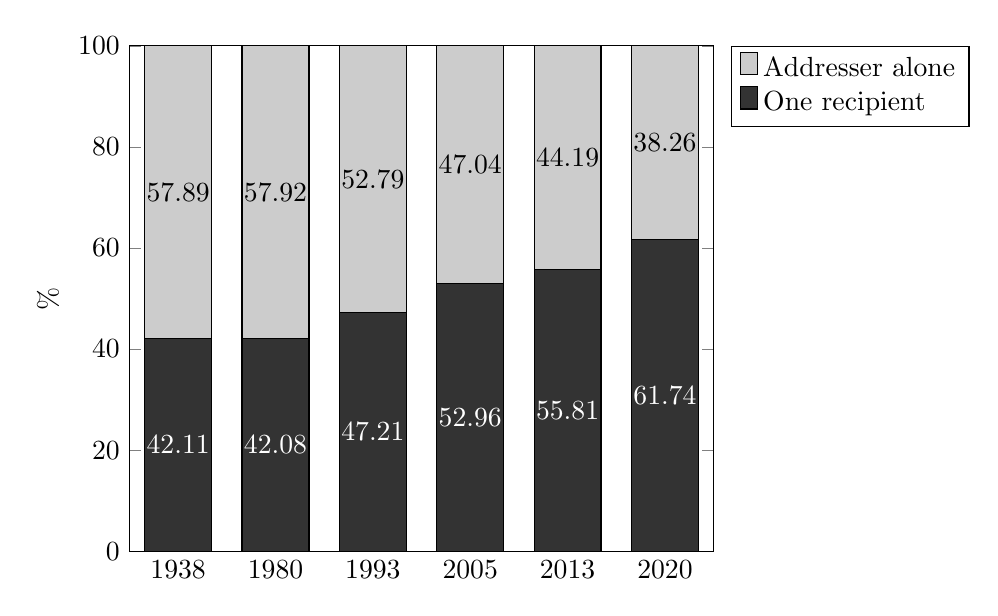
\begin{tikzpicture}
\pgfplotsset{compat=1.9}
\begin{axis}
	[
	ymin=0,
	ymax=100,
	ybar stacked,
	xtick=data,
	symbolic x coords={1938,1980,1993,2005,2013,2020},
	cycle list name=black white,
	bar width=.85cm,
	ylabel=\%,
	legend pos=outer north east,
	legend cell align=left,
	reverse legend=true,
	width=9cm,
	height=8cm
	]
	\addplot+ [fill=black!80,no markers,nodes near coords,nodes near coords style={color=white}] coordinates 
	   {(1938,42.11) 
		(1980,42.08)
		(1993,47.21)
		(2005,52.96)
		(2013,55.81)
		(2020,61.74)		
	};
	\addlegendentry{One recipient}
	\addplot+ [fill=black!20,no markers,nodes near coords] coordinates 
	   {(1938,57.89)
		(1980,57.92)
		(1993,52.79)
		(2005,47.04)
		(2013,44.19)
		(2020,38.26)		
	};
\addlegendentry{Addresser alone}
\end{axis}
\end{tikzpicture}
\end{figure}


If we focus on the evolution of the internal distribution of the reference to the addresser alone and the reference to one addressee (both addressed and unaddressed recipient), we also find a patterned evolution in the form of a linear regression (significance values calculated with ANOVA test, $p< 0.03$) (\figref{fig:nogue:2}): from more references to the addresser (in the 1932–1938 period and in 1980) to increasingly more references to the addressee (until 2005-20). Hence, as for individual reference, in the past MPs referred more to themselves than to other MPs, whereas now they refer more to other MPs than to themselves. Thus, the higher participant inscription we saw in \figref{fig:nogue:1} includes a tendency toward a more addressee-oriented reference, at least when the speaker’s discourse has a single recipient, either addressed or unaddressed. These data can be read as a patent rise in the interactivity of Catalan parliamentary debate. The fact that the general politics debate concerns the action of the Government, presented and defended by its President, can help explain such an increase in both absolute and relative terms (\citealt{DeCock2014}: 261–262).\largerpage

We focus now on the addresser reference and compare the reference to the speaker alone and the reference to the addresser groups (\figref{fig:nogue:3}). In this case, we can see a Pearson correlation in the data (significance values calculated with Pearson correlation, $p < 0.012$): the two variables show a similar amount of tokens for decades but, from 2013 onwards, they develop in opposite directions: the reference to the addresser groups grows while the reference to the speaker alone falls. That is, in the last decade, MPs, presidents and ministers include themselves in a group (the Government, the Parliament, the party, the country, and so on) more often than before, and at the same time they refer less and less to themselves alone. These figures seem to mirror an evolution in the conception of politics and government from a more individual to a more collective one.

\tabref{tab:nogue:17} includes the general quantitative results (both broken down into variables and global) without taking into account the 3\textsuperscript{rd} person strategies; \tabref{tab:nogue:18} includes the 3\textsuperscript{rd} person results; and \tabref{tab:nogue:19}, the changes in global data due to their incorporation in the analysis.\pagebreak

\begin{figure}[H]
\caption{The evolution of addresser-alone and addresser-group reference\label{fig:nogue:3}}
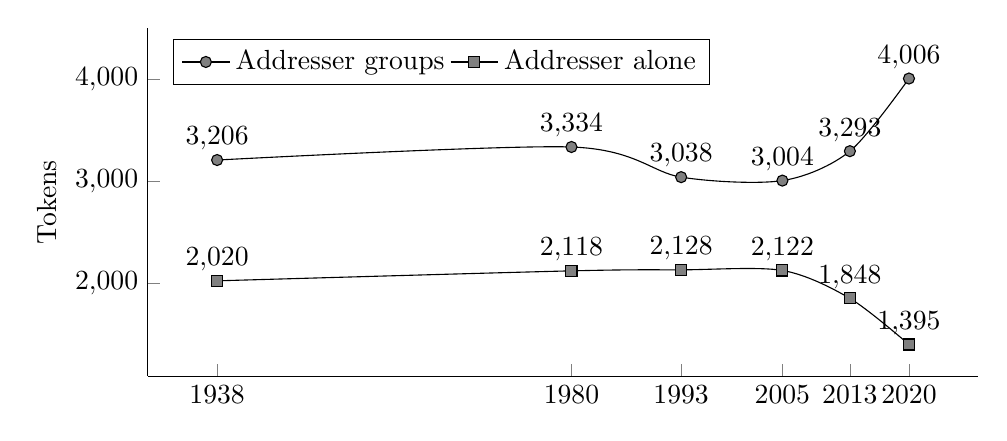
\begin{tikzpicture}
\begin{axis}
	[
	ymax=4500,
	width=\textwidth,
	height=6cm,
	axis lines*=left,
	legend pos=north west,
	legend columns=-1,
	xtick=data,
	x tick label style = {/pgf/number format/1000 sep={}},
	cycle list name=black white,
	smooth,
	ylabel={Tokens}
	]
	\addplot+ [nodes near coords] coordinates 
	   {(1938,3206)
		(1980,3334)
		(1993,3038)
		(2005,3004)
		(2013,3293)
		(2020,4006)		
	};
	\addlegendentry{Addresser groups}
	\addplot+ [nodes near coords] coordinates 
	{(1938,2020)
	(1980,2118)
	(1993,2128)
	(2005,2122)
	(2013,1848)
	(2020,1395)
	};
	\addlegendentry{Addresser alone}
\end{axis}
\end{tikzpicture}
\end{figure}\largerpage[2]


\begin{table}[H]
\small
\begin{tabular}{l *6{r}} 
\lsptoprule
& {1932–1938} & {1980} & {1993} & {2005} & {2013} & {2020}\\
\midrule
{1SG} & {2,129} & {2,070} & {2,119} & {2,081} & {1,839} & {1,380}\\
{1PL} & {2,377} & {2,965} & {2,754} & {2,543} & {3,037} & {3,816}\\
\midrule
{Total addresser} & {4,506} & {5,035} & {4,873} & {4,624} & {4,876} & {5,196}\\
\midrule
{\GlossMarkup{2SG} (informal)} & {0} & {10} & {9} & {26} & {80} & {34}\\
{\textit{Vós} (respectful)} & {40} & {4} & {366} & {0} & {0} & {0}\\
{\textit{Vostè} (formal)} & {4} & {312} & {858} & {1,388} & {1,712} & {1,588}\\
(\textit{la}) \textit{Vostra Senyoria} & {200} & {0} & {0} & {0} & {0} & {0}\\
{SG vocatives} & {62} & {237} & {260} & {232} & {348} & {269}\\
\midrule
{Total one recipient} & {306} & {563} & {1,493} & {1,646} & {2,140} & {1,891}\\
\midrule
\GlossMarkup{2PL} (\textit{tu} and \textit{vós})\footnote{(informal or respectful)} & {748} & {33} & {43} & {19} & {49} & {24}\\
{\textit{Vostès} (formal)} & {4} & {401} & {692} & {1,004} & {1,243} & {1,235}\\
(\textit{les}) \textit{Vostres\slash Ses Senyories} & {43} & {2} & {0} & {0} & {0} & {0}\\
{PL vocatives} & {92} & {70} & {63} & {62} & {57} & {51}\\
\midrule
{Total several recipients} & {887} & {506} & {798} & {1,085} & {1,349} & {1,310}\\
\midrule
{Total recipient(s)} & {1,193} & {1,069} & {2,291} & {2,731} & {3,489} & {3.201}\\
\midrule
{TOTAL} & {5,699} & {6,104} & {7,164} & {7,355} & {8,365} & {8,397}\\
\lspbottomrule
\end{tabular}
\caption{Global data without 3\textsuperscript{rd} person (number of tokens per 100,000 words)}
\label{tab:nogue:17}
\end{table}

\begin{table}[p]
\small
\begin{tabular}{llrrrrrr}
\lsptoprule
&              & 1932– & \\
& Reference to & {1938} & {1980} & {1993} & {2005} & {2013} & {{2020}}\\
\midrule
\GlossMarkup{3SG} & addresser & {71} & {48} & {9} & {41} & {9} & {15}\\
\GlossMarkup{3SG} & addresser groups & {782} & {348} & {268} & {429} & {250} & {180}\\
\GlossMarkup{3PL} & addresser groups & {47} & {21} & {16} & {32} & {6} & {10}\\
\midrule
\multicolumn{2}{l}{{Total} {3\textsuperscript{rd}} {person} {addresser}} & {{900}} & {{417}} & {{293}} & {{502}} & {{265}} & {{205}}\\
\midrule
\GlossMarkup{3SG} & one addressed recipient & {64} & {22} & {5} & {0} & {0} & {0}\\
\GlossMarkup{3SG} & one unaddressed recip. & {1,230} & {954} & {405} & {743} & {194} & {360}\\
\GlossMarkup{3SG} & a group of addr. recip. & {15} & {8} & {13} & {0} & {0} & {0}\\
\GlossMarkup{3SG} & a group of unaddr. recip. & {488} & {321} & {260} & {397} & {153} & {292}\\
\GlossMarkup{3PL} & a group of addr. recip. & {3} & {2} & {4} & {0} & {0} & {0}\\
\GlossMarkup{3PL} & a group of unaddr. recip. & {244} & {244} & {49} & {149} & {27} & {72}\\
\midrule
\multicolumn{2}{l}{{Total} {3\textsuperscript{rd}} {person} {addressee}} & {{2,044}} & {{1,551}} & {{736}} & {{1,289}} & {{374}} & {{724}}\\
\midrule
\multicolumn{2}{l}{{Total} {3\textsuperscript{rd}} {person} {strategies}} & {2,944} & {{1,968}} & {{1,029}} & {{1,791}} & {{639}} & {{929}}\\
\lspbottomrule
\end{tabular}
\caption{3\textsuperscript{rd} person strategies for the reference to the addresser and to the addressee(s) (number of tokens per 100,000 words)\label{tab:nogue:18}}
\end{table}

\begin{table}[p]
\small
\begin{tabular}{lcccccc} 
\lsptoprule
& {{1932–1938}} & {{1980}} & {{1993}} & {{2005}} & {{2013}} & {2020}\\
\midrule
{{Total} {addresser}} & {4,506} & {5,035} & {4,873} & {4,624} & {4,876} & {5,196}\\
{without} {3\textsuperscript{rd}} {person}\\
\midrule
{{Total} {addresser}} & {5,406} & {5,452} & {5,166} & {5,126} & {5,141} & {5,401}\\
{with} {3\textsuperscript{rd}} {person}\\
\midrule
{{Total} {recipient(s)}} & {1,193} & {1,069} & {2,291} & {2,731} & {3,489} & {3.201}\\
{without} {3\textsuperscript{rd}} {person}\\
\midrule
{{Total} {recipient(s)}} & {3,237} & {2,620} & {3,027} & {4,020} & {3,863} & {3,925}\\
{with} {3\textsuperscript{rd}} {person}\\
\midrule
{{Global} {data}} & {5,699} & {6,104} & {7,164} & {7,355} & {8,365} & {8,397}\\
{without} {3\textsuperscript{rd}} {person}\\
\midrule
{{Global} {data}} & {8,643} & {8,072} & {8,193} & {9,146} & {9,004} & {9,326}\\
{with} {3\textsuperscript{rd}} {person}\\
\lspbottomrule
\end{tabular}
\caption{Total addresser, total recipient(s) and global data without and with 3\textsuperscript{rd} person (number of tokens per 100,000 words)}
\label{tab:nogue:19}
\end{table}
\clearpage


The global data concerning the reference to the addresser and to the addresser groups reveal the following trends:


\begin{enumerate}
\item A slight global downward trend.

\item A clear increase in the preference for the inclusion in a group with a subsequent drop in the individual references to oneself, as we saw in \figref{fig:nogue:3}.

\item A gradual rise in the deictic forms of reference (in the 1\textsuperscript{st} person, SG or PL), more direct and less formal, to the exclusion of 3\textsuperscript{rd} person strategies, which are less direct and more formal.

\item In spite of the trend above, the 3\textsuperscript{rd} person strategy that has decreased the least is the use of the SG to refer to a group: mainly, the party, the parliamentary group or the Government.
\end{enumerate}


As for the reference to the recipient, a distinction must be made between references to addressed and to unaddressed recipients.



In the reference to the addressed recipient, the following trends are observed:

\begin{enumerate}

\item The disappearance of \textit{vós} in the present-day period. This form was only used systematically during the 1932–1938 period.

\item The disappearance in the present-day period of (\textit{la}) \textit{Vostra Senyoria}, which was also only used systematically during the 1932–1938 period, both in individual and collective references.

\item The decline of most 3\textsuperscript{rd} person non-prototypical strategies in the three last subcorpora (2005, 2013, and 2020). These strategies had been used during the 1932–1938 period, and some tokens are still found in 1980 and 1993. The evolution towards more direct and less formal forms is clear.

\item The systematic use of \textit{vostè(s)} in the present-day period, with a pronounced and sustained growth in both individual and collective references.

\item The sustained increase in the number of vocatives referring to a single recipient. Together with the introduction of more simple vocative forms in recent years (see \sectref{sec:nogue:2.2.1.6}), this growth illustrates once again the rising preference for more direct and less formal forms of reference.

\item The reduction in the number of vocatives referring to addressed recipient groups, which is compensated by the soaring use of \textit{vostè} just mentioned in 4.

\end{enumerate}

In the reference to the unaddressed recipient, the following trends are observed:

\begin{enumerate}

\item A general reduction in this kind of reference. Increasingly, MPs prefer to conceptualise the recipient, often a political adversary, as the addressed recipient, and they replace an indirect strategy of reference with a direct one: mainly \textit{vostè(s)}.

\item Within this overall trend, a smaller decrease is observed in the case of the reference to groups through a SG NP: political parties, parliamentary groups, Government…

\item A reduction, also smaller, in the case of the reference to a single unaddressed recipient is observed. The speech formula used by the President of the Parliament to give the floor to an addresser (\textit{Té la paraula el diputat / la diputada…} – ‘The MP… has the floor’) explains the maintenance of this strategy.
\end{enumerate}


Finally, the comparison of the global figures in Tables 17 and 18, summarised in \tabref{tab:nogue:19}, reveals straightforwardly how taking into account 3\textsuperscript{rd} person strategies for the analysis provides us with a more accurate view of the reality we want to describe and explain.


\tabref{tab:nogue:17} suggests a sustained increase in participant reference tokens, but \tabref{tab:nogue:19} shows that the real growth is much more moderate. It also shows a change in the preferred strategies: for the reference to the addresser, there is a trend towards the inclusion in groups to the detriment of individual references; for the reference to the recipient, and above all to the addressed recipient, over time we find a more reduced use of 3\textsuperscript{rd} person strategies, the decrease and later disappearance of the use of \textit{vós} and (\textit{la}) \textit{Vostra Senyoria}, and a surge in the use of \textit{vostè}(\textit{s}). \textit{Vostè}(\textit{s}) is also distant and formal, but it is a more direct strategy of reference than 3\textsuperscript{rd} person strategies.



\section{Conclusions}\label{sec:nogue:4}


Both the qualitative and the quantitative analyses of the corpus show that person deixis only (1\textsuperscript{st} and 2\textsuperscript{nd} person, including honorifics) is not enough to explain the reference to participants; the combination with \citegen{Goffman1981} participation frameworks allows the incorporation into the study of strategies for referring to unaddressed recipients. These strategies are added to other non-prototypical strategies of reference, also in the 3\textsuperscript{rd} person.

This first general conclusion, which is theoretical and methodological, goes beyond the study of participant reference in parliamentary debate and is highly relevant to an understanding of participant reference in general.

As for the specific results of the study, the conclusions can be summarised as follows:

\begin{enumerate}
\item Throughout the period analysed, the strategies for referring to the recipients (addressed and unaddressed) and the groups they belong to present a greater variety than those for referring to the addresser and the addresser groups.

\item From a structural point of view, vocatives evolve from more complex (\textit{Molt Honorable Senyor President}) to simpler forms (\textit{president}), and, from a functional point of view, from more formal and indirect to less formal and direct. The increase in the use of SG vocatives is related to the extension of more direct forms of reference to one recipient, and the reduction of PL vocatives can be explained by the extension of the use of \textit{vostès} and by a less frequent use of phatic \textit{(senyors) diputats / (senyores i senyors) diputats}.

\item The loss of \textit{vós} and (\textit{la}) \textit{Vostra Senyoria} (in SG and in PL), and the reduction of the use of 3\textsuperscript{rd} person forms, is compensated by the extension of the use of \textit{vostè}(\textit{s}). Hence, actually there is little variation in the total number of tokens of forms of participant reference, although a slight upward trend is observed. This growth also entails an increase in the degree of personalisation of the discourse of parliamentary debate.

\item These conclusions suggest that from the 1932–1938 period until now, and also within the present-day period, there is a major stylistic evolution from more indirect and formal strategies to more direct and less formal ones. This final conclusion is especially meaningful in an institutional setting, and it is consistent with wider processes that have affected many other registers of Catalan in that period, which can be summarised in a constant movement towards less formality within the continuum defined by the two extremes of solemnity (or the highest degree of formality, not absent from the parliamentary debate) and the most informal colloquiality (which would not be expected in this speech event).
\end{enumerate}

Two general questions, among others, remain open for further research. First, whether the movement towards less formality found in the Parliament of Catalonia is also found in other traditions of parliamentary discourse. Besides, it would be interesting to analyse to what extent this tendency is found in other genres of formal discourse, such as non-parliamentary political discourse, discourse of mass media, or academic discourse.

And second, whether participant reference in other parliamentary traditions presents the same properties and evolution. The different rules and uses found in the United Kingdom’s House of Commons, the Swedish Riksdag \citep{Ilie2010}, the Spanish Congreso de los Diputados (\citealt{DeCockNogué2017}), and the Parliament of Catalonia suggest that traditions regarding participant reference vary in several important aspects, and that contrastive analyses are needed to shed light upon the relation between these uses and the corresponding sociocultural contexts.


\section*{Abbreviations}\label{abbv:NogueSerrano}
The abbreviations used in the text follow the Leipzig Glossing Rules. Additional abbreviations for political parties, coalitions and parliamentary groups are:\medskip\\
% % % \subsection*{Linguistic terms}
% % %  NP = noun phrase
% % %  SG = singular
% % %  PL = plural
% % %  1SG = first person singular
% % %  2SG = second person singular
% % %  3SG = third person singular
% % %  1PL = first person plural
% % %  2PL = second person plural
% % %  3PL = third person plural.
% % % \subsection*{Political parties, coalitions and parliamentary groups}:
 \noindent\begin{tabular}{@{}ll@{}}
 CC-P & Catalunya en Comú Podem\\
 CC & Centristes de Catalunya\\
 C’s & Ciudadanos\\
 CUP & Candidatura d’Unitat Popular\\
 ERC & Esquerra Republicana de Catalunya\\
 CiU & Convergència i Unió\\
 GA & Grup Andalusista\\
 IC& Iniciativa per Catalunya\\
 ICV-EUA & Iniciativa per Catalunya Verds - Esquerra Unida i Alternativa\\
 Lliga & Lliga Regionalista/Lliga Catalana\\
 MP & Member of parliament\\
 PSC-PSOE & Partit dels Socialistes de Catalunya\\
 PSUC & Partit Socialista Unificat de Catalunya\\
 USC & Unió Socialista de Catalunya
 \end{tabular}
 
\section*{Comments and acknowledgments}
A previous version of this research was published in \citet{Nogué2018}. This revised, extended version includes a new subcorpus (updated to 2020) for both qualitative and quantitative analysis. In addition, a brief introduction to Catalan has been added. This chapter also includes a new section on the use of the first person singular in parliamentary debate (\sectref{sec:nogue:2.1}) and several minor updates to the previous version. We are deeply grateful to the anonymous reviewers for their suggestions and comments. This chapter is supported by the project \textit{Ambiguity at the grammar-pragmatics interface: structural and pragmatic factors} (reference PID2019-104453GA-I00), granted by the Spanish Ministerio de Ciencia, Innovación y Universidades to the Universitat de Barcelona.

\printbibliography[heading=subbibliography]
\end{document}
